\documentclass[twoside]{book}

% Packages required by doxygen
\usepackage{fixltx2e}
\usepackage{calc}
\usepackage{doxygen}
\usepackage[export]{adjustbox} % also loads graphicx
\usepackage{graphicx}
\usepackage[utf8]{inputenc}
\usepackage{makeidx}
\usepackage{multicol}
\usepackage{multirow}
\PassOptionsToPackage{warn}{textcomp}
\usepackage{textcomp}
\usepackage[nointegrals]{wasysym}
\usepackage[table]{xcolor}

% NLS support packages
\usepackage[spanish]{babel}
% Font selection
\usepackage[T1]{fontenc}
\usepackage[scaled=.90]{helvet}
\usepackage{courier}
\usepackage{amssymb}
\usepackage{sectsty}
\renewcommand{\familydefault}{\sfdefault}
\allsectionsfont{%
  \fontseries{bc}\selectfont%
  \color{darkgray}%
}
\renewcommand{\DoxyLabelFont}{%
  \fontseries{bc}\selectfont%
  \color{darkgray}%
}
\newcommand{\+}{\discretionary{\mbox{\scriptsize$\hookleftarrow$}}{}{}}

% Page & text layout
\usepackage{geometry}
\geometry{%
  a4paper,%
  top=2.5cm,%
  bottom=2.5cm,%
  left=2.5cm,%
  right=2.5cm%
}
\tolerance=750
\hfuzz=15pt
\hbadness=750
\setlength{\emergencystretch}{15pt}
\setlength{\parindent}{0cm}
\setlength{\parskip}{3ex plus 2ex minus 2ex}
\makeatletter
\renewcommand{\paragraph}{%
  \@startsection{paragraph}{4}{0ex}{-1.0ex}{1.0ex}{%
    \normalfont\normalsize\bfseries\SS@parafont%
  }%
}
\renewcommand{\subparagraph}{%
  \@startsection{subparagraph}{5}{0ex}{-1.0ex}{1.0ex}{%
    \normalfont\normalsize\bfseries\SS@subparafont%
  }%
}
\makeatother

% Headers & footers
\usepackage{fancyhdr}
\pagestyle{fancyplain}
\fancyhead[LE]{\fancyplain{}{\bfseries\thepage}}
\fancyhead[CE]{\fancyplain{}{}}
\fancyhead[RE]{\fancyplain{}{\bfseries\leftmark}}
\fancyhead[LO]{\fancyplain{}{\bfseries\rightmark}}
\fancyhead[CO]{\fancyplain{}{}}
\fancyhead[RO]{\fancyplain{}{\bfseries\thepage}}
\fancyfoot[LE]{\fancyplain{}{}}
\fancyfoot[CE]{\fancyplain{}{}}
\fancyfoot[RE]{\fancyplain{}{\bfseries\scriptsize Generado por Doxygen }}
\fancyfoot[LO]{\fancyplain{}{\bfseries\scriptsize Generado por Doxygen }}
\fancyfoot[CO]{\fancyplain{}{}}
\fancyfoot[RO]{\fancyplain{}{}}
\renewcommand{\footrulewidth}{0.4pt}
\renewcommand{\chaptermark}[1]{%
  \markboth{#1}{}%
}
\renewcommand{\sectionmark}[1]{%
  \markright{\thesection\ #1}%
}

% Indices & bibliography
\usepackage{natbib}
\usepackage[titles]{tocloft}
\setcounter{tocdepth}{3}
\setcounter{secnumdepth}{5}
\makeindex

% Hyperlinks (required, but should be loaded last)
\usepackage{ifpdf}
\ifpdf
  \usepackage[pdftex,pagebackref=true]{hyperref}
\else
  \usepackage[ps2pdf,pagebackref=true]{hyperref}
\fi
\hypersetup{%
  colorlinks=true,%
  linkcolor=blue,%
  citecolor=blue,%
  unicode%
}

% Custom commands
\newcommand{\clearemptydoublepage}{%
  \newpage{\pagestyle{empty}\cleardoublepage}%
}

\usepackage{caption}
\captionsetup{labelsep=space,justification=centering,font={bf},singlelinecheck=off,skip=4pt,position=top}

%===== C O N T E N T S =====

\begin{document}

% Titlepage & ToC
\hypersetup{pageanchor=false,
             bookmarksnumbered=true,
             pdfencoding=unicode
            }
\pagenumbering{roman}
\begin{titlepage}
\vspace*{7cm}
\begin{center}%
{\Large Laboratorio de P\+R\+O2. Experimentos en el laboratorio. \\[1ex]\large v1.\+0 18-\/05-\/2017 }\\
\vspace*{1cm}
{\large Generado por Doxygen 1.8.11}\\
\end{center}
\end{titlepage}
\clearemptydoublepage
\tableofcontents
\clearemptydoublepage
\pagenumbering{arabic}
\hypersetup{pageanchor=true}

%--- Begin generated contents ---
\chapter{Índice de clases}
\section{Llista de Classes}
Aquestes són les classes, estructures, unions i interfícies acompanyades amb breus descripcions\+:\begin{DoxyCompactList}
\item\contentsline{section}{\hyperlink{classindividu}{individu} }{\pageref{classindividu}}{}
\item\contentsline{section}{\hyperlink{classpoblacio}{poblacio} }{\pageref{classpoblacio}}{}
\end{DoxyCompactList}

\chapter{Indice de archivos}
\section{Llista dels Fitxers}
Aquesta és la llista de tots els fitxers acompanyats amb breus descripcions\+:\begin{DoxyCompactList}
\item\contentsline{section}{\hyperlink{especie_8cc}{especie.\+cc} \\*Codi de la clase especie }{\pageref{especie_8cc}}{}
\item\contentsline{section}{\hyperlink{especie_8hh}{especie.\+hh} \\*Especificació de la clase \hyperlink{especie_8hh}{especie.\+hh} }{\pageref{especie_8hh}}{}
\item\contentsline{section}{\hyperlink{individu_8cc}{individu.\+cc} \\*Codi de la clase individu }{\pageref{individu_8cc}}{}
\item\contentsline{section}{\hyperlink{individu_8hh}{individu.\+hh} \\*Especificació de la clase Individu }{\pageref{individu_8hh}}{}
\item\contentsline{section}{\hyperlink{parell__cromosomes_8cc}{parell\+\_\+cromosomes.\+cc} \\*Codi de la clase \hyperlink{classparell__cromosomes}{parell\+\_\+cromosomes} }{\pageref{parell__cromosomes_8cc}}{}
\item\contentsline{section}{\hyperlink{parell__cromosomes_8hh}{parell\+\_\+cromosomes.\+hh} \\*Especificació de la clase \hyperlink{classparell__cromosomes}{parell\+\_\+cromosomes} }{\pageref{parell__cromosomes_8hh}}{}
\item\contentsline{section}{\hyperlink{poblacio_8cc}{poblacio.\+cc} \\*Codi de la clase poblacio }{\pageref{poblacio_8cc}}{}
\item\contentsline{section}{\hyperlink{poblacio_8hh}{poblacio.\+hh} \\*Especificació de la clase poblacio }{\pageref{poblacio_8hh}}{}
\item\contentsline{section}{\hyperlink{program_8cc}{program.\+cc} }{\pageref{program_8cc}}{}
\end{DoxyCompactList}

\chapter{Documentación de las clases}
\hypertarget{classespecie}{}\section{Referència de la Classe especie}
\label{classespecie}\index{especie@{especie}}
\subsection*{Mètodes públics}
\begin{DoxyCompactItemize}
\item 
\hyperlink{classespecie_ac172ff6414744de38a9995de5b8960e6}{especie} ()
\item 
int \hyperlink{classespecie_a16cbac301660254cf39ef7f51690e507}{getN} ()
\begin{DoxyCompactList}\small\item\em Constructora de la clase especie. \end{DoxyCompactList}\item 
int \hyperlink{classespecie_ac09e154b4eae25155af3bdc98c2a18c3}{getl} (int i)
\begin{DoxyCompactList}\small\item\em Obtenir el nombre de cromosomes. \end{DoxyCompactList}\item 
int \hyperlink{classespecie_aeae1b17938e4527858ad4d3f5949d182}{getly} ()
\begin{DoxyCompactList}\small\item\em Obtenir la llargada del cromosoma C-\/i. \end{DoxyCompactList}\item 
int \hyperlink{classespecie_a98735feb10fd44e1316708566790ca95}{getlx} ()
\begin{DoxyCompactList}\small\item\em Obtenir la llargada del cromosoma sexual Y. \end{DoxyCompactList}\item 
int \hyperlink{classespecie_a5ea723fe64398cd46cbc6e044b114fff}{getl0} ()
\begin{DoxyCompactList}\small\item\em Obtenir la llargada del cromosoma sexual X. \end{DoxyCompactList}\item 
void \hyperlink{classespecie_af1a08ff40fdb79abb1d78c06b8131306}{llegir} ()
\begin{DoxyCompactList}\small\item\em Obtenir la part comuna dels cromosomes sexuals. \end{DoxyCompactList}\end{DoxyCompactItemize}


\subsection{Descripció Detallada}


Definició a la línia 1 del fitxer especie.\+hh.



\subsection{Documentació del Constructor i el Destructor}
\index{especie@{especie}!especie@{especie}}
\index{especie@{especie}!especie@{especie}}
\subsubsection[{\texorpdfstring{especie()}{especie()}}]{\setlength{\rightskip}{0pt plus 5cm}especie\+::especie (
\begin{DoxyParamCaption}
{}
\end{DoxyParamCaption}
)}\hypertarget{classespecie_ac172ff6414744de38a9995de5b8960e6}{}\label{classespecie_ac172ff6414744de38a9995de5b8960e6}


\subsection{Documentació de les Funcions Membre}
\index{especie@{especie}!getN@{getN}}
\index{getN@{getN}!especie@{especie}}
\subsubsection[{\texorpdfstring{get\+N()}{getN()}}]{\setlength{\rightskip}{0pt plus 5cm}int especie\+::getN (
\begin{DoxyParamCaption}
{}
\end{DoxyParamCaption}
)}\hypertarget{classespecie_a16cbac301660254cf39ef7f51690e507}{}\label{classespecie_a16cbac301660254cf39ef7f51690e507}


Constructora de la clase especie. 

\begin{DoxyPrecond}{Precondició}
Cert 
\end{DoxyPrecond}
\begin{DoxyPostcond}{Postcondició}
Obtenin una especie sense informació 
\end{DoxyPostcond}
\index{especie@{especie}!getl@{getl}}
\index{getl@{getl}!especie@{especie}}
\subsubsection[{\texorpdfstring{getl(int i)}{getl(int i)}}]{\setlength{\rightskip}{0pt plus 5cm}int especie\+::getl (
\begin{DoxyParamCaption}
\item[{int}]{i}
\end{DoxyParamCaption}
)}\hypertarget{classespecie_ac09e154b4eae25155af3bdc98c2a18c3}{}\label{classespecie_ac09e154b4eae25155af3bdc98c2a18c3}


Obtenir el nombre de cromosomes. 

\begin{DoxyPrecond}{Precondició}
Cert 
\end{DoxyPrecond}
\begin{DoxyPostcond}{Postcondició}
El valor retornat es N (nombre de cromosomes) 
\end{DoxyPostcond}
\index{especie@{especie}!getly@{getly}}
\index{getly@{getly}!especie@{especie}}
\subsubsection[{\texorpdfstring{getly()}{getly()}}]{\setlength{\rightskip}{0pt plus 5cm}int especie\+::getly (
\begin{DoxyParamCaption}
{}
\end{DoxyParamCaption}
)}\hypertarget{classespecie_aeae1b17938e4527858ad4d3f5949d182}{}\label{classespecie_aeae1b17938e4527858ad4d3f5949d182}


Obtenir la llargada del cromosoma C-\/i. 

\begin{DoxyPrecond}{Precondició}
el p.\+i es la posició del cromosoma 
\end{DoxyPrecond}
\begin{DoxyPostcond}{Postcondició}
El valor retornat es la llargada del cromosoma c-\/i 
\end{DoxyPostcond}
\index{especie@{especie}!getlx@{getlx}}
\index{getlx@{getlx}!especie@{especie}}
\subsubsection[{\texorpdfstring{getlx()}{getlx()}}]{\setlength{\rightskip}{0pt plus 5cm}int especie\+::getlx (
\begin{DoxyParamCaption}
{}
\end{DoxyParamCaption}
)}\hypertarget{classespecie_a98735feb10fd44e1316708566790ca95}{}\label{classespecie_a98735feb10fd44e1316708566790ca95}


Obtenir la llargada del cromosoma sexual Y. 

\begin{DoxyPrecond}{Precondició}
Cert 
\end{DoxyPrecond}
\begin{DoxyPostcond}{Postcondició}
El valor retornat es la llargada del cromosoma sexual Y 
\end{DoxyPostcond}
\index{especie@{especie}!getl0@{getl0}}
\index{getl0@{getl0}!especie@{especie}}
\subsubsection[{\texorpdfstring{getl0()}{getl0()}}]{\setlength{\rightskip}{0pt plus 5cm}int especie\+::getl0 (
\begin{DoxyParamCaption}
{}
\end{DoxyParamCaption}
)}\hypertarget{classespecie_a5ea723fe64398cd46cbc6e044b114fff}{}\label{classespecie_a5ea723fe64398cd46cbc6e044b114fff}


Obtenir la llargada del cromosoma sexual X. 

\begin{DoxyPrecond}{Precondició}
Cert 
\end{DoxyPrecond}
\begin{DoxyPostcond}{Postcondició}
El valor retornat es la llargada del cromosoma sexual X 
\end{DoxyPostcond}
\index{especie@{especie}!llegir@{llegir}}
\index{llegir@{llegir}!especie@{especie}}
\subsubsection[{\texorpdfstring{llegir()}{llegir()}}]{\setlength{\rightskip}{0pt plus 5cm}void especie\+::llegir (
\begin{DoxyParamCaption}
{}
\end{DoxyParamCaption}
)}\hypertarget{classespecie_af1a08ff40fdb79abb1d78c06b8131306}{}\label{classespecie_af1a08ff40fdb79abb1d78c06b8131306}


Obtenir la part comuna dels cromosomes sexuals. 

\begin{DoxyPrecond}{Precondició}
cert 
\end{DoxyPrecond}
\begin{DoxyPostcond}{Postcondició}
Retornem el parametre l0 
\end{DoxyPostcond}


La documentació d\textquotesingle{}aquesta classe es va generar a partir del següent fitxer\+:\begin{DoxyCompactItemize}
\item 
\hyperlink{especie_8hh}{especie.\+hh}\end{DoxyCompactItemize}

\hypertarget{structpoblacio_1_1familia}{}\section{Referència de l\textquotesingle{}Estructura poblacio\+:\+:familia}
\label{structpoblacio_1_1familia}\index{poblacio\+::familia@{poblacio\+::familia}}


Estructura familia amb iteradors que apunten al pare i a la mare de l\textquotesingle{}individu.  


\subsection*{Atributs Públics}
\begin{DoxyCompactItemize}
\item 
\hyperlink{classindividu}{individu} \hyperlink{structpoblacio_1_1familia_a184e9fe52d7cf62ca133ac1d900f87ea}{in}
\begin{DoxyCompactList}\small\item\em L\textquotesingle{}individu emmagatzemat en el sistema. \end{DoxyCompactList}\item 
map$<$ string, \hyperlink{structpoblacio_1_1familia}{familia} $>$\+::iterator \hyperlink{structpoblacio_1_1familia_af87f56b016ade8b4bb02a49036de5f74}{pare}
\begin{DoxyCompactList}\small\item\em L\textquotesingle{}iterador que apunta al seu pare. \end{DoxyCompactList}\item 
map$<$ string, \hyperlink{structpoblacio_1_1familia}{familia} $>$\+::iterator \hyperlink{structpoblacio_1_1familia_a9d44bf543d7f856a93feac40de233c42}{mare}
\begin{DoxyCompactList}\small\item\em L\textquotesingle{}iterador que apunta a la seva mare. \end{DoxyCompactList}\end{DoxyCompactItemize}


\subsection{Descripció Detallada}
Estructura familia amb iteradors que apunten al pare i a la mare de l\textquotesingle{}individu. 

Definició a la línia 26 del fitxer poblacio.\+hh.



\subsection{Documentació de les Dades Membre}
\index{poblacio\+::familia@{poblacio\+::familia}!in@{in}}
\index{in@{in}!poblacio\+::familia@{poblacio\+::familia}}
\subsubsection[{\texorpdfstring{in}{in}}]{\setlength{\rightskip}{0pt plus 5cm}{\bf individu} poblacio\+::familia\+::in}\hypertarget{structpoblacio_1_1familia_a184e9fe52d7cf62ca133ac1d900f87ea}{}\label{structpoblacio_1_1familia_a184e9fe52d7cf62ca133ac1d900f87ea}


L\textquotesingle{}individu emmagatzemat en el sistema. 



Definició a la línia 31 del fitxer poblacio.\+hh.

\index{poblacio\+::familia@{poblacio\+::familia}!pare@{pare}}
\index{pare@{pare}!poblacio\+::familia@{poblacio\+::familia}}
\subsubsection[{\texorpdfstring{pare}{pare}}]{\setlength{\rightskip}{0pt plus 5cm}map$<$string,{\bf familia}$>$\+::iterator poblacio\+::familia\+::pare}\hypertarget{structpoblacio_1_1familia_af87f56b016ade8b4bb02a49036de5f74}{}\label{structpoblacio_1_1familia_af87f56b016ade8b4bb02a49036de5f74}


L\textquotesingle{}iterador que apunta al seu pare. 



Definició a la línia 33 del fitxer poblacio.\+hh.

\index{poblacio\+::familia@{poblacio\+::familia}!mare@{mare}}
\index{mare@{mare}!poblacio\+::familia@{poblacio\+::familia}}
\subsubsection[{\texorpdfstring{mare}{mare}}]{\setlength{\rightskip}{0pt plus 5cm}map$<$string,{\bf familia}$>$\+::iterator poblacio\+::familia\+::mare}\hypertarget{structpoblacio_1_1familia_a9d44bf543d7f856a93feac40de233c42}{}\label{structpoblacio_1_1familia_a9d44bf543d7f856a93feac40de233c42}


L\textquotesingle{}iterador que apunta a la seva mare. 



Definició a la línia 35 del fitxer poblacio.\+hh.



La documentació d\textquotesingle{}aquesta estructura es va generar a partir del següent fitxer\+:\begin{DoxyCompactItemize}
\item 
\hyperlink{poblacio_8hh}{poblacio.\+hh}\end{DoxyCompactItemize}

\hypertarget{structfamilia}{}\section{Referencia de la Estructura familia}
\label{structfamilia}\index{familia@{familia}}


Estructura on emmagetzem l\textquotesingle{}individu, i el seu pare i la mare.  




\subsection{Descripción detallada}
Estructura on emmagetzem l\textquotesingle{}individu, i el seu pare i la mare. 

La documentación para esta estructura fue generada a partir del siguiente fichero\+:\begin{DoxyCompactItemize}
\item 
\hyperlink{poblacio_8hh}{poblacio.\+hh}\end{DoxyCompactItemize}

\hypertarget{classindividu}{}\section{Referència de la Classe individu}
\label{classindividu}\index{individu@{individu}}
\subsection*{Mètodes públics}
\begin{DoxyCompactItemize}
\item 
\hyperlink{classindividu_af1ba9dc86a04bff6b41ed2d1cf3202b9}{individu} ()
\begin{DoxyCompactList}\small\item\em Definim els parametres de la especie per a tots els individus. \end{DoxyCompactList}\item 
\hyperlink{classindividu_ad05b5a1094b6b85e3704bee2d9de4717}{individu} (\hyperlink{classindividu}{individu} pare, \hyperlink{classindividu}{individu} mare, string nfill)
\begin{DoxyCompactList}\small\item\em Generem un individu buit. \end{DoxyCompactList}\item 
void \hyperlink{classindividu_afe94f6bc70378a3b7607e99bd4b260f2}{comprovararbre} (Arbre$<$ string $>$ arb)
\begin{DoxyCompactList}\small\item\em Retornem un individu nou, fill del pare i la mare mitjançant la reproducció \end{DoxyCompactList}\item 
void \hyperlink{classindividu_a25a2d30b548c13a92bb2cbeacebc722c}{consultarnom} ()
\begin{DoxyCompactList}\small\item\em Comprovem que un arbre es subarbre de l\textquotesingle{}arbre geneologic del individu. \end{DoxyCompactList}\item 
void \hyperlink{classindividu_aef8e17be688e7e31270d5207aa008587}{sexe} ()
\begin{DoxyCompactList}\small\item\em Escribim el nom de l\textquotesingle{}individu. \end{DoxyCompactList}\item 
void \hyperlink{classindividu_ad7b6f532a96228f4ba7b9a948d7051c9}{pares} ()
\begin{DoxyCompactList}\small\item\em Escribim el sexe de l\textquotesingle{}individu. \end{DoxyCompactList}\item 
void \hyperlink{classindividu_a48da0b7cc9612b7854668377b591fdd7}{llegir} ()
\begin{DoxyCompactList}\small\item\em Escribim els pares de l\textquotesingle{}individu. \end{DoxyCompactList}\item 
void \hyperlink{classindividu_ab65a6fb5fabbddcedfc56fb70efdbe55}{familia} ()
\begin{DoxyCompactList}\small\item\em Llegim un individu. \end{DoxyCompactList}\item 
void \hyperlink{classindividu_a88659e52840409422fc354b513ca03a8}{escriure} ()
\begin{DoxyCompactList}\small\item\em Escribim la familia de l\textquotesingle{}individu. \end{DoxyCompactList}\end{DoxyCompactItemize}
\subsection*{Mètodes Públics Estàtics}
\begin{DoxyCompactItemize}
\item 
static void \hyperlink{classindividu_aafe8b7748069bd4801b546dbffb1570d}{definir} (int N, int li, int lx, int ly)
\end{DoxyCompactItemize}


\subsection{Descripció Detallada}


Definició a la línia 6 del fitxer individu.\+hh.



\subsection{Documentació del Constructor i el Destructor}
\index{individu@{individu}!individu@{individu}}
\index{individu@{individu}!individu@{individu}}
\subsubsection[{\texorpdfstring{individu()}{individu()}}]{\setlength{\rightskip}{0pt plus 5cm}individu\+::individu (
\begin{DoxyParamCaption}
{}
\end{DoxyParamCaption}
)}\hypertarget{classindividu_af1ba9dc86a04bff6b41ed2d1cf3202b9}{}\label{classindividu_af1ba9dc86a04bff6b41ed2d1cf3202b9}


Definim els parametres de la especie per a tots els individus. 

\begin{DoxyPrecond}{Precondició}
Al P.\+I tenim N (nombre de cromosomes), li (longitud d\textquotesingle{}ells) i ly, lx (longitud dels sexuals) 
\end{DoxyPrecond}
\begin{DoxyPostcond}{Postcondició}
Aquets P.\+I pasen a ser els atributs de tots els individus 
\end{DoxyPostcond}
\index{individu@{individu}!individu@{individu}}
\index{individu@{individu}!individu@{individu}}
\subsubsection[{\texorpdfstring{individu(individu pare, individu mare, string nfill)}{individu(individu pare, individu mare, string nfill)}}]{\setlength{\rightskip}{0pt plus 5cm}individu\+::individu (
\begin{DoxyParamCaption}
\item[{{\bf individu}}]{pare, }
\item[{{\bf individu}}]{mare, }
\item[{string}]{nfill}
\end{DoxyParamCaption}
)}\hypertarget{classindividu_ad05b5a1094b6b85e3704bee2d9de4717}{}\label{classindividu_ad05b5a1094b6b85e3704bee2d9de4717}


Generem un individu buit. 

\begin{DoxyPrecond}{Precondició}
buit 
\end{DoxyPrecond}
\begin{DoxyPostcond}{Postcondició}
Retornem un individu buit 
\end{DoxyPostcond}


\subsection{Documentació de les Funcions Membre}
\index{individu@{individu}!definir@{definir}}
\index{definir@{definir}!individu@{individu}}
\subsubsection[{\texorpdfstring{definir(int N, int li, int lx, int ly)}{definir(int N, int li, int lx, int ly)}}]{\setlength{\rightskip}{0pt plus 5cm}static void individu\+::definir (
\begin{DoxyParamCaption}
\item[{int}]{N, }
\item[{int}]{li, }
\item[{int}]{lx, }
\item[{int}]{ly}
\end{DoxyParamCaption}
)\hspace{0.3cm}{\ttfamily [static]}}\hypertarget{classindividu_aafe8b7748069bd4801b546dbffb1570d}{}\label{classindividu_aafe8b7748069bd4801b546dbffb1570d}
\index{individu@{individu}!comprovararbre@{comprovararbre}}
\index{comprovararbre@{comprovararbre}!individu@{individu}}
\subsubsection[{\texorpdfstring{comprovararbre(\+Arbre$<$ string $>$ arb)}{comprovararbre(Arbre< string > arb)}}]{\setlength{\rightskip}{0pt plus 5cm}void individu\+::comprovararbre (
\begin{DoxyParamCaption}
\item[{Arbre$<$ string $>$}]{arb}
\end{DoxyParamCaption}
)}\hypertarget{classindividu_afe94f6bc70378a3b7607e99bd4b260f2}{}\label{classindividu_afe94f6bc70378a3b7607e99bd4b260f2}


Retornem un individu nou, fill del pare i la mare mitjançant la reproducció 

\begin{DoxyPrecond}{Precondició}
Al P.\+I estan el pare, la mare i el nom del fill (on pare XY, mare XX) 
\end{DoxyPrecond}
\begin{DoxyPostcond}{Postcondició}
Retornem un individu nou mitjançant la reproduccio 
\end{DoxyPostcond}
\index{individu@{individu}!consultarnom@{consultarnom}}
\index{consultarnom@{consultarnom}!individu@{individu}}
\subsubsection[{\texorpdfstring{consultarnom()}{consultarnom()}}]{\setlength{\rightskip}{0pt plus 5cm}void individu\+::consultarnom (
\begin{DoxyParamCaption}
{}
\end{DoxyParamCaption}
)}\hypertarget{classindividu_a25a2d30b548c13a92bb2cbeacebc722c}{}\label{classindividu_a25a2d30b548c13a92bb2cbeacebc722c}


Comprovem que un arbre es subarbre de l\textquotesingle{}arbre geneologic del individu. 

\begin{DoxyPrecond}{Precondició}
arb es un arbre 
\end{DoxyPrecond}
\begin{DoxyPostcond}{Postcondició}
s\textquotesingle{}han escrit al canal estandard de sortida si arb es subarbre dels arbre geneologic del individu 
\end{DoxyPostcond}
\index{individu@{individu}!sexe@{sexe}}
\index{sexe@{sexe}!individu@{individu}}
\subsubsection[{\texorpdfstring{sexe()}{sexe()}}]{\setlength{\rightskip}{0pt plus 5cm}void individu\+::sexe (
\begin{DoxyParamCaption}
{}
\end{DoxyParamCaption}
)}\hypertarget{classindividu_aef8e17be688e7e31270d5207aa008587}{}\label{classindividu_aef8e17be688e7e31270d5207aa008587}


Escribim el nom de l\textquotesingle{}individu. 

\begin{DoxyPrecond}{Precondició}
buit 
\end{DoxyPrecond}
\begin{DoxyPostcond}{Postcondició}
S\textquotesingle{}ha escrit el nom de l\textquotesingle{}individu al canal estandard de sortida 
\end{DoxyPostcond}
\index{individu@{individu}!pares@{pares}}
\index{pares@{pares}!individu@{individu}}
\subsubsection[{\texorpdfstring{pares()}{pares()}}]{\setlength{\rightskip}{0pt plus 5cm}void individu\+::pares (
\begin{DoxyParamCaption}
{}
\end{DoxyParamCaption}
)}\hypertarget{classindividu_ad7b6f532a96228f4ba7b9a948d7051c9}{}\label{classindividu_ad7b6f532a96228f4ba7b9a948d7051c9}


Escribim el sexe de l\textquotesingle{}individu. 

\begin{DoxyPrecond}{Precondició}
buit 
\end{DoxyPrecond}
\begin{DoxyPostcond}{Postcondició}
S\textquotesingle{}ha escrit el sexe de l\textquotesingle{}individu al canal estandard de sortida 
\end{DoxyPostcond}
\index{individu@{individu}!llegir@{llegir}}
\index{llegir@{llegir}!individu@{individu}}
\subsubsection[{\texorpdfstring{llegir()}{llegir()}}]{\setlength{\rightskip}{0pt plus 5cm}void individu\+::llegir (
\begin{DoxyParamCaption}
{}
\end{DoxyParamCaption}
)}\hypertarget{classindividu_a48da0b7cc9612b7854668377b591fdd7}{}\label{classindividu_a48da0b7cc9612b7854668377b591fdd7}


Escribim els pares de l\textquotesingle{}individu. 

\begin{DoxyPrecond}{Precondició}
buit 
\end{DoxyPrecond}
\begin{DoxyPostcond}{Postcondició}
S\textquotesingle{}han escrit els pares de l\textquotesingle{}individu al canal estandard de sortida 
\end{DoxyPostcond}
\index{individu@{individu}!familia@{familia}}
\index{familia@{familia}!individu@{individu}}
\subsubsection[{\texorpdfstring{familia()}{familia()}}]{\setlength{\rightskip}{0pt plus 5cm}void individu\+::familia (
\begin{DoxyParamCaption}
{}
\end{DoxyParamCaption}
)}\hypertarget{classindividu_ab65a6fb5fabbddcedfc56fb70efdbe55}{}\label{classindividu_ab65a6fb5fabbddcedfc56fb70efdbe55}


Llegim un individu. 

\begin{DoxyPrecond}{Precondició}
Al canal estandard d\textquotesingle{}entrada tenim les dades de un individu, l\textquotesingle{}individu es buit 
\end{DoxyPrecond}
\begin{DoxyPostcond}{Postcondició}
Assignem els valors que rebem al individus 
\end{DoxyPostcond}
\index{individu@{individu}!escriure@{escriure}}
\index{escriure@{escriure}!individu@{individu}}
\subsubsection[{\texorpdfstring{escriure()}{escriure()}}]{\setlength{\rightskip}{0pt plus 5cm}void individu\+::escriure (
\begin{DoxyParamCaption}
{}
\end{DoxyParamCaption}
)}\hypertarget{classindividu_a88659e52840409422fc354b513ca03a8}{}\label{classindividu_a88659e52840409422fc354b513ca03a8}


Escribim la familia de l\textquotesingle{}individu. 

\begin{DoxyPrecond}{Precondició}
buit 
\end{DoxyPrecond}
\begin{DoxyPostcond}{Postcondició}
S\textquotesingle{}ha escrit la familia de l\textquotesingle{}individu al canal estandard de sortida 
\end{DoxyPostcond}


La documentació d\textquotesingle{}aquesta classe es va generar a partir del següent fitxer\+:\begin{DoxyCompactItemize}
\item 
\hyperlink{individu_8hh}{individu.\+hh}\end{DoxyCompactItemize}

\hypertarget{classparell__cromosomes}{}\section{Referència de la Classe parell\+\_\+cromosomes}
\label{classparell__cromosomes}\index{parell\+\_\+cromosomes@{parell\+\_\+cromosomes}}


Emmagatzema la informacio de un parell de cromosomes amb metodes per a fer posible la reproduccio i escriure els genotips.  


\subsection*{Mètodes públics}
\begin{DoxyCompactItemize}
\item 
\hyperlink{classparell__cromosomes_a9d86452d029f65ccf80c8861c4914698}{parell\+\_\+cromosomes} ()
\begin{DoxyCompactList}\small\item\em constructora del parell de cromosomes \end{DoxyCompactList}\item 
\hyperlink{classparell__cromosomes_aa7f0798619677ef4715f2d94ecd39769}{parell\+\_\+cromosomes} (const vector$<$ bool $>$ \&\hyperlink{classparell__cromosomes_ab4d7cfc40f53a1698b4ea3ef1f2cd199}{c1}, const vector$<$ bool $>$ \&\hyperlink{classparell__cromosomes_a888f09ecbc3329b0ee505fb0cb8bf98f}{c2})
\begin{DoxyCompactList}\small\item\em constructora del parell de cromosomes \end{DoxyCompactList}\item 
void \hyperlink{classparell__cromosomes_a3192f21452f2885d61032eb547cb4a15}{tallar} (int i)
\item 
vector$<$ bool $>$ \hyperlink{classparell__cromosomes_a25cf02baa8f399adc798289773729b5e}{consultar\+\_\+c1} () const 
\begin{DoxyCompactList}\small\item\em llegim el parell de cromosomes \end{DoxyCompactList}\item 
vector$<$ bool $>$ \hyperlink{classparell__cromosomes_a4c29928abe72237272e5e1e219dc3e9d}{consultar\+\_\+c2} () const 
\begin{DoxyCompactList}\small\item\em Retornem el cromosoma c2. \end{DoxyCompactList}\item 
void \hyperlink{classparell__cromosomes_a3217cc5eb83e77521b28f091c7cf5a5a}{llegir} (int tam)
\begin{DoxyCompactList}\small\item\em Tallem els cromosomes. \end{DoxyCompactList}\item 
void \hyperlink{classparell__cromosomes_a1bd9e226b1fe9d3e02302e9230c8b928}{escriure\+\_\+c1} ()
\begin{DoxyCompactList}\small\item\em Escribim el cromosoma c1. \end{DoxyCompactList}\item 
void \hyperlink{classparell__cromosomes_a109c96b0eb5e9c63ec97fa0b1e62c252}{escriure\+\_\+c2} ()
\begin{DoxyCompactList}\small\item\em Escribim el cromosoma c2. \end{DoxyCompactList}\end{DoxyCompactItemize}
\subsection*{Atributs Privats}
\begin{DoxyCompactItemize}
\item 
vector$<$ bool $>$ \hyperlink{classparell__cromosomes_ab4d7cfc40f53a1698b4ea3ef1f2cd199}{c1}
\begin{DoxyCompactList}\small\item\em vector que representa el cromosoma 1 \end{DoxyCompactList}\item 
vector$<$ bool $>$ \hyperlink{classparell__cromosomes_a888f09ecbc3329b0ee505fb0cb8bf98f}{c2}
\begin{DoxyCompactList}\small\item\em vector que representa el cromosoma 2 \end{DoxyCompactList}\end{DoxyCompactItemize}


\subsection{Descripció Detallada}
Emmagatzema la informacio de un parell de cromosomes amb metodes per a fer posible la reproduccio i escriure els genotips. 

Definició a la línia 11 del fitxer parell\+\_\+cromosomes.\+hh.



\subsection{Documentació del Constructor i el Destructor}
\index{parell\+\_\+cromosomes@{parell\+\_\+cromosomes}!parell\+\_\+cromosomes@{parell\+\_\+cromosomes}}
\index{parell\+\_\+cromosomes@{parell\+\_\+cromosomes}!parell\+\_\+cromosomes@{parell\+\_\+cromosomes}}
\subsubsection[{\texorpdfstring{parell\+\_\+cromosomes()}{parell_cromosomes()}}]{\setlength{\rightskip}{0pt plus 5cm}parell\+\_\+cromosomes\+::parell\+\_\+cromosomes (
\begin{DoxyParamCaption}
{}
\end{DoxyParamCaption}
)}\hypertarget{classparell__cromosomes_a9d86452d029f65ccf80c8861c4914698}{}\label{classparell__cromosomes_a9d86452d029f65ccf80c8861c4914698}


constructora del parell de cromosomes 

\begin{DoxyPrecond}{Precondició}
cert 
\end{DoxyPrecond}
\begin{DoxyPostcond}{Postcondició}
Retornem un parell de cromosomes buit 
\end{DoxyPostcond}


Definició a la línia 8 del fitxer parell\+\_\+cromosomes.\+cc.


\begin{DoxyCode}
8                                     \{
9 
10 \}
\end{DoxyCode}
\index{parell\+\_\+cromosomes@{parell\+\_\+cromosomes}!parell\+\_\+cromosomes@{parell\+\_\+cromosomes}}
\index{parell\+\_\+cromosomes@{parell\+\_\+cromosomes}!parell\+\_\+cromosomes@{parell\+\_\+cromosomes}}
\subsubsection[{\texorpdfstring{parell\+\_\+cromosomes(const vector$<$ bool $>$ \&c1, const vector$<$ bool $>$ \&c2)}{parell_cromosomes(const vector< bool > &c1, const vector< bool > &c2)}}]{\setlength{\rightskip}{0pt plus 5cm}parell\+\_\+cromosomes\+::parell\+\_\+cromosomes (
\begin{DoxyParamCaption}
\item[{const vector$<$ bool $>$ \&}]{c1, }
\item[{const vector$<$ bool $>$ \&}]{c2}
\end{DoxyParamCaption}
)}\hypertarget{classparell__cromosomes_aa7f0798619677ef4715f2d94ecd39769}{}\label{classparell__cromosomes_aa7f0798619677ef4715f2d94ecd39769}


constructora del parell de cromosomes 

\begin{DoxyPrecond}{Precondició}
c1 i c2 son cromosomes 
\end{DoxyPrecond}
\begin{DoxyPostcond}{Postcondició}
Retornem un parell de cromosomes on el P.\+I son els cromosomes 
\end{DoxyPostcond}


Definició a la línia 12 del fitxer parell\+\_\+cromosomes.\+cc.


\begin{DoxyCode}
12                                                                                \{
13     (*this).c1 = \hyperlink{classparell__cromosomes_ab4d7cfc40f53a1698b4ea3ef1f2cd199}{c1};
14 
15     (*this).c2 = \hyperlink{classparell__cromosomes_a888f09ecbc3329b0ee505fb0cb8bf98f}{c2};
16 \}
\end{DoxyCode}


\subsection{Documentació de les Funcions Membre}
\index{parell\+\_\+cromosomes@{parell\+\_\+cromosomes}!tallar@{tallar}}
\index{tallar@{tallar}!parell\+\_\+cromosomes@{parell\+\_\+cromosomes}}
\subsubsection[{\texorpdfstring{tallar(int i)}{tallar(int i)}}]{\setlength{\rightskip}{0pt plus 5cm}void parell\+\_\+cromosomes\+::tallar (
\begin{DoxyParamCaption}
\item[{int}]{i}
\end{DoxyParamCaption}
)}\hypertarget{classparell__cromosomes_a3192f21452f2885d61032eb547cb4a15}{}\label{classparell__cromosomes_a3192f21452f2885d61032eb547cb4a15}


Definició a la línia 19 del fitxer parell\+\_\+cromosomes.\+cc.


\begin{DoxyCode}
19                                    \{
20     
21   \textcolor{comment}{//intercambiem els valors de i fins a size}
22   \textcolor{keywordflow}{for}(\textcolor{keywordtype}{int} j = i; j<\hyperlink{classparell__cromosomes_ab4d7cfc40f53a1698b4ea3ef1f2cd199}{c1}.size(); ++j)\{
23     \textcolor{keywordtype}{bool} aux;       \textcolor{comment}{//}
24     aux = \hyperlink{classparell__cromosomes_ab4d7cfc40f53a1698b4ea3ef1f2cd199}{c1}[j];    \textcolor{comment}{//}
25     \hyperlink{classparell__cromosomes_ab4d7cfc40f53a1698b4ea3ef1f2cd199}{c1}[j] = \hyperlink{classparell__cromosomes_a888f09ecbc3329b0ee505fb0cb8bf98f}{c2}[j];  \textcolor{comment}{//swap}
26     \hyperlink{classparell__cromosomes_a888f09ecbc3329b0ee505fb0cb8bf98f}{c2}[j] = aux;    \textcolor{comment}{//}
27 
28   \}
29 \}
\end{DoxyCode}
\index{parell\+\_\+cromosomes@{parell\+\_\+cromosomes}!consultar\+\_\+c1@{consultar\+\_\+c1}}
\index{consultar\+\_\+c1@{consultar\+\_\+c1}!parell\+\_\+cromosomes@{parell\+\_\+cromosomes}}
\subsubsection[{\texorpdfstring{consultar\+\_\+c1() const }{consultar_c1() const }}]{\setlength{\rightskip}{0pt plus 5cm}vector$<$ bool $>$ parell\+\_\+cromosomes\+::consultar\+\_\+c1 (
\begin{DoxyParamCaption}
{}
\end{DoxyParamCaption}
) const}\hypertarget{classparell__cromosomes_a25cf02baa8f399adc798289773729b5e}{}\label{classparell__cromosomes_a25cf02baa8f399adc798289773729b5e}


llegim el parell de cromosomes 

\begin{DoxyPrecond}{Precondició}
al canal estandard d\textquotesingle{}entrada esta la sequencia de gens dels dos cromosomes 
\end{DoxyPrecond}
\begin{DoxyPostcond}{Postcondició}
cr1 i cr2 han quedat definits\+Retornem el cromosoma c1 
\end{DoxyPostcond}
\begin{DoxyPrecond}{Precondició}
cert 
\end{DoxyPrecond}
\begin{DoxyPostcond}{Postcondició}
retornem el cromosoma c1 
\end{DoxyPostcond}


Definició a la línia 32 del fitxer parell\+\_\+cromosomes.\+cc.


\begin{DoxyCode}
32                                                   \{
33     \textcolor{keywordflow}{return} \hyperlink{classparell__cromosomes_ab4d7cfc40f53a1698b4ea3ef1f2cd199}{c1};
34 \}
\end{DoxyCode}
\index{parell\+\_\+cromosomes@{parell\+\_\+cromosomes}!consultar\+\_\+c2@{consultar\+\_\+c2}}
\index{consultar\+\_\+c2@{consultar\+\_\+c2}!parell\+\_\+cromosomes@{parell\+\_\+cromosomes}}
\subsubsection[{\texorpdfstring{consultar\+\_\+c2() const }{consultar_c2() const }}]{\setlength{\rightskip}{0pt plus 5cm}vector$<$ bool $>$ parell\+\_\+cromosomes\+::consultar\+\_\+c2 (
\begin{DoxyParamCaption}
{}
\end{DoxyParamCaption}
) const}\hypertarget{classparell__cromosomes_a4c29928abe72237272e5e1e219dc3e9d}{}\label{classparell__cromosomes_a4c29928abe72237272e5e1e219dc3e9d}


Retornem el cromosoma c2. 

\begin{DoxyPrecond}{Precondició}
cert 
\end{DoxyPrecond}
\begin{DoxyPostcond}{Postcondició}
retornem el cromosoma c2 
\end{DoxyPostcond}


Definició a la línia 36 del fitxer parell\+\_\+cromosomes.\+cc.


\begin{DoxyCode}
36                                                   \{
37     \textcolor{keywordflow}{return} \hyperlink{classparell__cromosomes_a888f09ecbc3329b0ee505fb0cb8bf98f}{c2};
38 \}
\end{DoxyCode}
\index{parell\+\_\+cromosomes@{parell\+\_\+cromosomes}!llegir@{llegir}}
\index{llegir@{llegir}!parell\+\_\+cromosomes@{parell\+\_\+cromosomes}}
\subsubsection[{\texorpdfstring{llegir(int tam)}{llegir(int tam)}}]{\setlength{\rightskip}{0pt plus 5cm}void parell\+\_\+cromosomes\+::llegir (
\begin{DoxyParamCaption}
\item[{int}]{tam}
\end{DoxyParamCaption}
)}\hypertarget{classparell__cromosomes_a3217cc5eb83e77521b28f091c7cf5a5a}{}\label{classparell__cromosomes_a3217cc5eb83e77521b28f091c7cf5a5a}


Tallem els cromosomes. 

\begin{DoxyPrecond}{Precondició}
0$<$i$<$li 
\end{DoxyPrecond}
\begin{DoxyPostcond}{Postcondició}
retornem el cromosoma c2 
\end{DoxyPostcond}


Definició a la línia 41 del fitxer parell\+\_\+cromosomes.\+cc.


\begin{DoxyCode}
41                                      \{
42     \textcolor{comment}{//inicialitzem els cromosomes}
43     \hyperlink{classparell__cromosomes_ab4d7cfc40f53a1698b4ea3ef1f2cd199}{c1} = vector<bool>(tam);
44     \hyperlink{classparell__cromosomes_a888f09ecbc3329b0ee505fb0cb8bf98f}{c2} = vector<bool>(tam);
45     \textcolor{keywordtype}{int} inp;
46     
47     \textcolor{comment}{//llegim el primer cromosoma}
48     \textcolor{keywordflow}{for}(\textcolor{keywordtype}{int} i = 0; i<tam; ++i)\{
49         cin>>inp;
50         \hyperlink{classparell__cromosomes_ab4d7cfc40f53a1698b4ea3ef1f2cd199}{c1}[i] = inp;
51     \}
52     
53     \textcolor{comment}{//llegim el segon cromosoma}
54     \textcolor{keywordflow}{for}(\textcolor{keywordtype}{int} i = 0; i<tam; ++i)\{
55         cin>>inp;
56         c2[i] = inp;
57     \}
58 \}
\end{DoxyCode}
\index{parell\+\_\+cromosomes@{parell\+\_\+cromosomes}!escriure\+\_\+c1@{escriure\+\_\+c1}}
\index{escriure\+\_\+c1@{escriure\+\_\+c1}!parell\+\_\+cromosomes@{parell\+\_\+cromosomes}}
\subsubsection[{\texorpdfstring{escriure\+\_\+c1()}{escriure_c1()}}]{\setlength{\rightskip}{0pt plus 5cm}void parell\+\_\+cromosomes\+::escriure\+\_\+c1 (
\begin{DoxyParamCaption}
{}
\end{DoxyParamCaption}
)}\hypertarget{classparell__cromosomes_a1bd9e226b1fe9d3e02302e9230c8b928}{}\label{classparell__cromosomes_a1bd9e226b1fe9d3e02302e9230c8b928}


Escribim el cromosoma c1. 

\begin{DoxyPrecond}{Precondició}
cert 
\end{DoxyPrecond}
\begin{DoxyPostcond}{Postcondició}
El canal estandard de sortida ha quedat escrit amb la sequencia de gens del cromosoma c1 
\end{DoxyPostcond}


Definició a la línia 60 del fitxer parell\+\_\+cromosomes.\+cc.


\begin{DoxyCode}
60                                    \{
61     cout<<\textcolor{stringliteral}{"1:"};
62     \textcolor{keywordflow}{for}(\textcolor{keywordtype}{int} i = 0; i<\hyperlink{classparell__cromosomes_ab4d7cfc40f53a1698b4ea3ef1f2cd199}{c1}.size(); ++i)\{
63         cout<<\textcolor{stringliteral}{" "};
64         \textcolor{keywordflow}{if}(\hyperlink{classparell__cromosomes_ab4d7cfc40f53a1698b4ea3ef1f2cd199}{c1}[i])cout<<\textcolor{stringliteral}{"1"};
65         \textcolor{keywordflow}{else} cout<<\textcolor{stringliteral}{"0"};
66     \}
67 \}
\end{DoxyCode}
\index{parell\+\_\+cromosomes@{parell\+\_\+cromosomes}!escriure\+\_\+c2@{escriure\+\_\+c2}}
\index{escriure\+\_\+c2@{escriure\+\_\+c2}!parell\+\_\+cromosomes@{parell\+\_\+cromosomes}}
\subsubsection[{\texorpdfstring{escriure\+\_\+c2()}{escriure_c2()}}]{\setlength{\rightskip}{0pt plus 5cm}void parell\+\_\+cromosomes\+::escriure\+\_\+c2 (
\begin{DoxyParamCaption}
{}
\end{DoxyParamCaption}
)}\hypertarget{classparell__cromosomes_a109c96b0eb5e9c63ec97fa0b1e62c252}{}\label{classparell__cromosomes_a109c96b0eb5e9c63ec97fa0b1e62c252}


Escribim el cromosoma c2. 

\begin{DoxyPrecond}{Precondició}
cert 
\end{DoxyPrecond}
\begin{DoxyPostcond}{Postcondició}
El canal estandard de sortida ha quedat escrit amb la sequencia de gens del cromosoma c2 
\end{DoxyPostcond}


Definició a la línia 69 del fitxer parell\+\_\+cromosomes.\+cc.


\begin{DoxyCode}
69                                    \{
70     cout<<\textcolor{stringliteral}{"2:"};
71     \textcolor{keywordflow}{for}(\textcolor{keywordtype}{int} i = 0; i<\hyperlink{classparell__cromosomes_a888f09ecbc3329b0ee505fb0cb8bf98f}{c2}.size(); ++i)\{
72         cout<<\textcolor{stringliteral}{" "};
73         \textcolor{keywordflow}{if}(\hyperlink{classparell__cromosomes_a888f09ecbc3329b0ee505fb0cb8bf98f}{c2}[i])cout<<\textcolor{stringliteral}{"1"};
74         \textcolor{keywordflow}{else} cout<<\textcolor{stringliteral}{"0"};
75     \}
76 \}
\end{DoxyCode}


\subsection{Documentació de les Dades Membre}
\index{parell\+\_\+cromosomes@{parell\+\_\+cromosomes}!c1@{c1}}
\index{c1@{c1}!parell\+\_\+cromosomes@{parell\+\_\+cromosomes}}
\subsubsection[{\texorpdfstring{c1}{c1}}]{\setlength{\rightskip}{0pt plus 5cm}vector$<$bool$>$ parell\+\_\+cromosomes\+::c1\hspace{0.3cm}{\ttfamily [private]}}\hypertarget{classparell__cromosomes_ab4d7cfc40f53a1698b4ea3ef1f2cd199}{}\label{classparell__cromosomes_ab4d7cfc40f53a1698b4ea3ef1f2cd199}


vector que representa el cromosoma 1 



Definició a la línia 17 del fitxer parell\+\_\+cromosomes.\+hh.

\index{parell\+\_\+cromosomes@{parell\+\_\+cromosomes}!c2@{c2}}
\index{c2@{c2}!parell\+\_\+cromosomes@{parell\+\_\+cromosomes}}
\subsubsection[{\texorpdfstring{c2}{c2}}]{\setlength{\rightskip}{0pt plus 5cm}vector$<$bool$>$ parell\+\_\+cromosomes\+::c2\hspace{0.3cm}{\ttfamily [private]}}\hypertarget{classparell__cromosomes_a888f09ecbc3329b0ee505fb0cb8bf98f}{}\label{classparell__cromosomes_a888f09ecbc3329b0ee505fb0cb8bf98f}


vector que representa el cromosoma 2 



Definició a la línia 19 del fitxer parell\+\_\+cromosomes.\+hh.



La documentació d\textquotesingle{}aquesta classe es va generar a partir dels següents fitxers\+:\begin{DoxyCompactItemize}
\item 
\hyperlink{parell__cromosomes_8hh}{parell\+\_\+cromosomes.\+hh}\item 
\hyperlink{parell__cromosomes_8cc}{parell\+\_\+cromosomes.\+cc}\end{DoxyCompactItemize}

\hypertarget{classpoblacio}{}\section{Referència de la Classe poblacio}
\label{classpoblacio}\index{poblacio@{poblacio}}


sistema on emmagatzemem els individus amb el seu nom i un iterador que apunta al pare i la mare de cada individu.  


\subsection*{Classes}
\begin{DoxyCompactItemize}
\item 
struct \hyperlink{structpoblacio_1_1familia}{familia}
\begin{DoxyCompactList}\small\item\em Estructura familia amb iteradors que apunten al pare i a la mare de l\textquotesingle{}individu. \end{DoxyCompactList}\end{DoxyCompactItemize}
\subsection*{Mètodes públics}
\begin{DoxyCompactItemize}
\item 
\hyperlink{classpoblacio_a8d6ad7ce285dd47c9cfd806e302d7086}{poblacio} ()
\begin{DoxyCompactList}\small\item\em Retorna una poblacio buida. \end{DoxyCompactList}\item 
void \hyperlink{classpoblacio_a09a516141a9a8bef9249239916894af5}{afegir\+\_\+individu} (string nom, const \hyperlink{classindividu}{individu} \&ind)
\begin{DoxyCompactList}\small\item\em Afegim un individu al map pob. \end{DoxyCompactList}\item 
void \hyperlink{classpoblacio_a347bc063088e161813c257211d8059b9}{reproduir} (string pare, string mare, string fill, \hyperlink{classespecie}{especie} \&esp)
\begin{DoxyCompactList}\small\item\em reproduim dos individus i si es posible l\textquotesingle{}afegim al sistema \end{DoxyCompactList}\item 
bool \hyperlink{classpoblacio_a9c6fe58f2cbd06574070df2ef4076015}{esta\+\_\+individu} (string nom)
\begin{DoxyCompactList}\small\item\em Busquem un individu al sistema. \end{DoxyCompactList}\item 
void \hyperlink{classpoblacio_a1e30be9019dcb194171228c41284117f}{completar\+\_\+arbre} ()
\begin{DoxyCompactList}\small\item\em llegim un arbre diem si es o no subarbre de l\textquotesingle{}arbre geneologic d\textquotesingle{}algun individu i si ho es el completem marcant els nous \end{DoxyCompactList}\item 
bool \hyperlink{classpoblacio_a0002a245d187017cf1af34b364c176a0}{son\+\_\+antecesors} (string a, string b)
\begin{DoxyCompactList}\small\item\em Busquem si els elements son antecesors. \end{DoxyCompactList}\item 
\hyperlink{classindividu}{individu} \hyperlink{classpoblacio_a30ec7988306978a608ab11062069e6e1}{consultar\+\_\+individu} (string nom)
\begin{DoxyCompactList}\small\item\em Consultem un individu. \end{DoxyCompactList}\item 
void \hyperlink{classpoblacio_a02fda63e8b0144ce197764753778a201}{llegir} (\hyperlink{classespecie}{especie} \&esp)
\begin{DoxyCompactList}\small\item\em Llegim una població inicial. \end{DoxyCompactList}\item 
void \hyperlink{classpoblacio_aef82aca848d299bc5eff6d6b479a5081}{escriure} ()
\begin{DoxyCompactList}\small\item\em Escribim tots els elements per ordre alfabetic. \end{DoxyCompactList}\item 
void \hyperlink{classpoblacio_a30e1c829999a403012ce09172461d656}{escriure\+\_\+arbre\+\_\+geneologic} (string nom)
\begin{DoxyCompactList}\small\item\em Escribim l\textquotesingle{}arbre geneologic de l\textquotesingle{}individu. \end{DoxyCompactList}\end{DoxyCompactItemize}
\subsection*{Tipus Privats}
\begin{DoxyCompactItemize}
\item 
typedef map$<$ string, \hyperlink{structpoblacio_1_1familia}{familia} $>$\+::iterator \hyperlink{classpoblacio_a52c3d96b08f7679f27487e7499185ed1}{mapiterator}
\begin{DoxyCompactList}\small\item\em Typedef per a amenitzar la programacio. \end{DoxyCompactList}\end{DoxyCompactItemize}
\subsection*{Mètodes Privats}
\begin{DoxyCompactItemize}
\item 
bool \hyperlink{classpoblacio_ad8651d82e2eb8863e853d57d9b8b9985}{reproduccio\+\_\+posible} (\hyperlink{classpoblacio_a52c3d96b08f7679f27487e7499185ed1}{mapiterator} pare, \hyperlink{classpoblacio_a52c3d96b08f7679f27487e7499185ed1}{mapiterator} mare, \hyperlink{classpoblacio_a52c3d96b08f7679f27487e7499185ed1}{mapiterator} fill)
\begin{DoxyCompactList}\small\item\em diem si es posible la reproduccio, metode privat ja que treballem amb mapiteradors. \end{DoxyCompactList}\item 
bool \hyperlink{classpoblacio_a03e79690411d8ca8aa7d1e5646ca1c19}{te\+\_\+pares} (\hyperlink{classpoblacio_a52c3d96b08f7679f27487e7499185ed1}{mapiterator} a)
\begin{DoxyCompactList}\small\item\em Retorna cert si l\textquotesingle{}individu te pares operacio privada ja que treballem amb mapiterator. \end{DoxyCompactList}\item 
bool \hyperlink{classpoblacio_a068248eaa6d1090e4114e2c799c850b1}{es\+\_\+antecesor\+\_\+aux} (\hyperlink{classpoblacio_a52c3d96b08f7679f27487e7499185ed1}{mapiterator} low, string high)
\begin{DoxyCompactList}\small\item\em Retorna cert si el nom de l\textquotesingle{}individu high es un antecesor de l\textquotesingle{}individu low operacio privada ja que treballem amb mapiterator\textquotesingle{}s. \end{DoxyCompactList}\item 
void \hyperlink{classpoblacio_a90b5d501f5b346aecb3c1ba170b3fb6f}{completar} (queue$<$ string $>$ \&to\+\_\+print, \hyperlink{classpoblacio_a52c3d96b08f7679f27487e7499185ed1}{mapiterator} actual)
\begin{DoxyCompactList}\small\item\em Donada una cua i un mapiterador, la plenem completant l\textquotesingle{}arbre geneolofic de l\textquotesingle{}individu actual. \end{DoxyCompactList}\item 
bool \hyperlink{classpoblacio_a85493b733f10c8a276986a5a32404352}{completar\+\_\+arbre\+\_\+aux} (queue$<$ string $>$ \&to\+\_\+print, \hyperlink{classpoblacio_a52c3d96b08f7679f27487e7499185ed1}{mapiterator} actual)
\begin{DoxyCompactList}\small\item\em Retorna cert si donat un arbre en preordre es subarbre de l\textquotesingle{}inidividu actual, a mes a mes, el completem. \end{DoxyCompactList}\end{DoxyCompactItemize}
\subsection*{Atributs Privats}
\begin{DoxyCompactItemize}
\item 
map$<$ string, \hyperlink{structpoblacio_1_1familia}{familia} $>$ \hyperlink{classpoblacio_a7ecb70033b151a937143b07d489c4c17}{pob}
\begin{DoxyCompactList}\small\item\em Mapa on guardem els individus amb els seus noms. \end{DoxyCompactList}\end{DoxyCompactItemize}


\subsection{Descripció Detallada}
sistema on emmagatzemem els individus amb el seu nom i un iterador que apunta al pare i la mare de cada individu. 

Les operacions que tracten amb iteradors les em declarat com a privades 

Definició a la línia 15 del fitxer poblacio.\+hh.



\subsection{Documentació de les Definicions de Tipus Membre}
\index{poblacio@{poblacio}!mapiterator@{mapiterator}}
\index{mapiterator@{mapiterator}!poblacio@{poblacio}}
\subsubsection[{\texorpdfstring{mapiterator}{mapiterator}}]{\setlength{\rightskip}{0pt plus 5cm}typedef map$<$string,{\bf familia}$>$\+::iterator {\bf poblacio\+::mapiterator}\hspace{0.3cm}{\ttfamily [private]}}\hypertarget{classpoblacio_a52c3d96b08f7679f27487e7499185ed1}{}\label{classpoblacio_a52c3d96b08f7679f27487e7499185ed1}


Typedef per a amenitzar la programacio. 



Definició a la línia 42 del fitxer poblacio.\+hh.



\subsection{Documentació del Constructor i el Destructor}
\index{poblacio@{poblacio}!poblacio@{poblacio}}
\index{poblacio@{poblacio}!poblacio@{poblacio}}
\subsubsection[{\texorpdfstring{poblacio()}{poblacio()}}]{\setlength{\rightskip}{0pt plus 5cm}poblacio\+::poblacio (
\begin{DoxyParamCaption}
{}
\end{DoxyParamCaption}
)}\hypertarget{classpoblacio_a8d6ad7ce285dd47c9cfd806e302d7086}{}\label{classpoblacio_a8d6ad7ce285dd47c9cfd806e302d7086}


Retorna una poblacio buida. 

\begin{DoxyPrecond}{Precondició}
cert 
\end{DoxyPrecond}
\begin{DoxyPostcond}{Postcondició}
Retornem una poblacio buida 
\end{DoxyPostcond}


Definició a la línia 113 del fitxer poblacio.\+cc.


\begin{DoxyCode}
113                   \{
114 
115 \}
\end{DoxyCode}


\subsection{Documentació de les Funcions Membre}
\index{poblacio@{poblacio}!reproduccio\+\_\+posible@{reproduccio\+\_\+posible}}
\index{reproduccio\+\_\+posible@{reproduccio\+\_\+posible}!poblacio@{poblacio}}
\subsubsection[{\texorpdfstring{reproduccio\+\_\+posible(mapiterator pare, mapiterator mare, mapiterator fill)}{reproduccio_posible(mapiterator pare, mapiterator mare, mapiterator fill)}}]{\setlength{\rightskip}{0pt plus 5cm}bool poblacio\+::reproduccio\+\_\+posible (
\begin{DoxyParamCaption}
\item[{{\bf mapiterator}}]{pare, }
\item[{{\bf mapiterator}}]{mare, }
\item[{{\bf mapiterator}}]{fill}
\end{DoxyParamCaption}
)\hspace{0.3cm}{\ttfamily [private]}}\hypertarget{classpoblacio_ad8651d82e2eb8863e853d57d9b8b9985}{}\label{classpoblacio_ad8651d82e2eb8863e853d57d9b8b9985}


diem si es posible la reproduccio, metode privat ja que treballem amb mapiteradors. 

\begin{DoxyPrecond}{Precondició}
cert 
\end{DoxyPrecond}
\begin{DoxyPostcond}{Postcondició}
retornem cert si la reproduccio es posible i fals si no, a demes a quedat escrit el tipus de error 
\end{DoxyPostcond}


Definició a la línia 9 del fitxer poblacio.\+cc.


\begin{DoxyCode}
9                                                                                       \{
10     \textcolor{comment}{//comprovem que pare i mare estiguin al sistema,i que el fill no hi sigui}
11     \textcolor{keywordflow}{if}(pare == \hyperlink{classpoblacio_a7ecb70033b151a937143b07d489c4c17}{pob}.end() or mare == \hyperlink{classpoblacio_a7ecb70033b151a937143b07d489c4c17}{pob}.end() or fill !=\hyperlink{classpoblacio_a7ecb70033b151a937143b07d489c4c17}{pob}.end())\{
12       cout<<\textcolor{stringliteral}{"  error"}<<endl;
13       \textcolor{keywordflow}{return} \textcolor{keyword}{false};
14     \}
15 
16     \textcolor{comment}{//Comprobem els sexes del pare i la mare}
17     \textcolor{keywordflow}{if}((*pare).second.in.consultar\_sexe() or !(*mare).second.in.consultar\_sexe())\{
18       cout<<\textcolor{stringliteral}{"  no es posible reproduccion"}<<endl;
19       \textcolor{keywordflow}{return} \textcolor{keyword}{false};
20     \}
21 
22     \textcolor{comment}{//mirem que no siguin germans (no tinguin ni el mateix pare ni la mateixa mare)}
23     \hyperlink{classpoblacio_a52c3d96b08f7679f27487e7499185ed1}{mapiterator} avip = (*pare).second.pare;
24     \hyperlink{classpoblacio_a52c3d96b08f7679f27487e7499185ed1}{mapiterator} avim = (*mare).second.pare;
25     \hyperlink{classpoblacio_a52c3d96b08f7679f27487e7499185ed1}{mapiterator} aviap = (*pare).second.mare;
26     \hyperlink{classpoblacio_a52c3d96b08f7679f27487e7499185ed1}{mapiterator} aviam = (*mare).second.mare;
27 
28     \textcolor{keywordflow}{if}(avip != \hyperlink{classpoblacio_a7ecb70033b151a937143b07d489c4c17}{pob}.end() and avim != \hyperlink{classpoblacio_a7ecb70033b151a937143b07d489c4c17}{pob}.end())\{
29       \textcolor{keywordflow}{if}((*avip).first == (*avim).first)\{
30         cout<<\textcolor{stringliteral}{"  no es posible reproduccion"}<<endl;
31         \textcolor{keywordflow}{return} \textcolor{keyword}{false};
32       \}
33     \}
34 
35     \textcolor{keywordflow}{if}(aviap != \hyperlink{classpoblacio_a7ecb70033b151a937143b07d489c4c17}{pob}.end() and aviam != \hyperlink{classpoblacio_a7ecb70033b151a937143b07d489c4c17}{pob}.end())\{
36       \textcolor{keywordflow}{if}((*aviap).first == (*aviam).first)\{
37         cout<<\textcolor{stringliteral}{"  no es posible reproduccion"}<<endl;
38         \textcolor{keywordflow}{return} \textcolor{keyword}{false};
39       \}
40     \}
41 
42     \textcolor{comment}{//finalment mirem que un no sigui antecesor de l'altre i viceversa}
43     \textcolor{keywordflow}{if}(\hyperlink{classpoblacio_a0002a245d187017cf1af34b364c176a0}{son\_antecesors}((*pare).first, (*mare).first))\{
44       cout<<\textcolor{stringliteral}{"  no es posible reproduccion"}<<endl;
45       \textcolor{keywordflow}{return} \textcolor{keyword}{false};
46     \}
47     \textcolor{comment}{//si compleix totes les condicions retornem cert}
48     \textcolor{keywordflow}{return} \textcolor{keyword}{true};
49 
50 \}
\end{DoxyCode}
\index{poblacio@{poblacio}!te\+\_\+pares@{te\+\_\+pares}}
\index{te\+\_\+pares@{te\+\_\+pares}!poblacio@{poblacio}}
\subsubsection[{\texorpdfstring{te\+\_\+pares(mapiterator a)}{te_pares(mapiterator a)}}]{\setlength{\rightskip}{0pt plus 5cm}bool poblacio\+::te\+\_\+pares (
\begin{DoxyParamCaption}
\item[{{\bf mapiterator}}]{a}
\end{DoxyParamCaption}
)\hspace{0.3cm}{\ttfamily [private]}}\hypertarget{classpoblacio_a03e79690411d8ca8aa7d1e5646ca1c19}{}\label{classpoblacio_a03e79690411d8ca8aa7d1e5646ca1c19}


Retorna cert si l\textquotesingle{}individu te pares operacio privada ja que treballem amb mapiterator. 

\begin{DoxyPrecond}{Precondició}
cert 
\end{DoxyPrecond}
\begin{DoxyPostcond}{Postcondició}
Retornem cert si l\textquotesingle{}individu apuntat per el mapiterator te pares 
\end{DoxyPostcond}


Definició a la línia 52 del fitxer poblacio.\+cc.


\begin{DoxyCode}
52                                     \{
53   \textcolor{keywordflow}{return} (*a).second.pare != \hyperlink{classpoblacio_a7ecb70033b151a937143b07d489c4c17}{pob}.end();
54 \}
\end{DoxyCode}
\index{poblacio@{poblacio}!es\+\_\+antecesor\+\_\+aux@{es\+\_\+antecesor\+\_\+aux}}
\index{es\+\_\+antecesor\+\_\+aux@{es\+\_\+antecesor\+\_\+aux}!poblacio@{poblacio}}
\subsubsection[{\texorpdfstring{es\+\_\+antecesor\+\_\+aux(mapiterator low, string high)}{es_antecesor_aux(mapiterator low, string high)}}]{\setlength{\rightskip}{0pt plus 5cm}bool poblacio\+::es\+\_\+antecesor\+\_\+aux (
\begin{DoxyParamCaption}
\item[{{\bf mapiterator}}]{low, }
\item[{string}]{high}
\end{DoxyParamCaption}
)\hspace{0.3cm}{\ttfamily [private]}}\hypertarget{classpoblacio_a068248eaa6d1090e4114e2c799c850b1}{}\label{classpoblacio_a068248eaa6d1090e4114e2c799c850b1}


Retorna cert si el nom de l\textquotesingle{}individu high es un antecesor de l\textquotesingle{}individu low operacio privada ja que treballem amb mapiterator\textquotesingle{}s. 

\begin{DoxyPrecond}{Precondició}
cert 
\end{DoxyPrecond}
\begin{DoxyPostcond}{Postcondició}
Retornem cert si l\textquotesingle{}individu al qual correspon el nom high es antecesor de low. 
\end{DoxyPostcond}


Definició a la línia 56 del fitxer poblacio.\+cc.


\begin{DoxyCode}
56                                                            \{
57       \textcolor{keywordtype}{bool} b;
58       \textcolor{keywordflow}{if}(low == this->\hyperlink{classpoblacio_a7ecb70033b151a937143b07d489c4c17}{pob}.end()) b = \textcolor{keyword}{false}; \textcolor{comment}{//si no el trobem retornem fals}
59       \textcolor{keywordflow}{else} b = ((*low).first == high or \hyperlink{classpoblacio_a068248eaa6d1090e4114e2c799c850b1}{es\_antecesor\_aux}((*low).second.pare, high) or 
      \hyperlink{classpoblacio_a068248eaa6d1090e4114e2c799c850b1}{es\_antecesor\_aux}((*low).second.mare, high));
60       \textcolor{comment}{//^si el nom es igual al que busquem retornem cert i no fem les crides recursives i sino doncs mirem
       a partir del pare i despres de la mare}
61     return b;
62 \}
\end{DoxyCode}
\index{poblacio@{poblacio}!completar@{completar}}
\index{completar@{completar}!poblacio@{poblacio}}
\subsubsection[{\texorpdfstring{completar(queue$<$ string $>$ \&to\+\_\+print, mapiterator actual)}{completar(queue< string > &to_print, mapiterator actual)}}]{\setlength{\rightskip}{0pt plus 5cm}void poblacio\+::completar (
\begin{DoxyParamCaption}
\item[{queue$<$ string $>$ \&}]{to\+\_\+print, }
\item[{{\bf mapiterator}}]{actual}
\end{DoxyParamCaption}
)\hspace{0.3cm}{\ttfamily [private]}}\hypertarget{classpoblacio_a90b5d501f5b346aecb3c1ba170b3fb6f}{}\label{classpoblacio_a90b5d501f5b346aecb3c1ba170b3fb6f}


Donada una cua i un mapiterador, la plenem completant l\textquotesingle{}arbre geneolofic de l\textquotesingle{}individu actual. 

\begin{DoxyPrecond}{Precondició}
cert 
\end{DoxyPrecond}
\begin{DoxyPostcond}{Postcondició}
to\+\_\+print ha quedat plenada amb l\textquotesingle{}arbre geneologic de l\textquotesingle{}individu 
\end{DoxyPostcond}


Definició a la línia 64 del fitxer poblacio.\+cc.


\begin{DoxyCode}
64                                                                   \{
65       \textcolor{keywordflow}{if}(actual != \hyperlink{classpoblacio_a7ecb70033b151a937143b07d489c4c17}{pob}.end())\{
66         \textcolor{comment}{//afegim lelement a la cua entre asteriscs per a imprimirlo com a nou}
67         to\_print.push(\textcolor{stringliteral}{"*"}+(*actual).first+\textcolor{stringliteral}{"*"});
68         \textcolor{comment}{//realitzem crides recursives per al pare i la mare respectant el preordre}
69         (*this).completar(to\_print, (*actual).second.pare);
70         (*this).completar(to\_print, (*actual).second.mare);
71       \}\textcolor{keywordflow}{else}\{
72         \textcolor{comment}{//si es un valor null afegil un $ i aturem les crides recursives (cas base)}
73         to\_print.push(\textcolor{stringliteral}{"$"});
74       \}
75 \}
\end{DoxyCode}
\index{poblacio@{poblacio}!completar\+\_\+arbre\+\_\+aux@{completar\+\_\+arbre\+\_\+aux}}
\index{completar\+\_\+arbre\+\_\+aux@{completar\+\_\+arbre\+\_\+aux}!poblacio@{poblacio}}
\subsubsection[{\texorpdfstring{completar\+\_\+arbre\+\_\+aux(queue$<$ string $>$ \&to\+\_\+print, mapiterator actual)}{completar_arbre_aux(queue< string > &to_print, mapiterator actual)}}]{\setlength{\rightskip}{0pt plus 5cm}bool poblacio\+::completar\+\_\+arbre\+\_\+aux (
\begin{DoxyParamCaption}
\item[{queue$<$ string $>$ \&}]{to\+\_\+print, }
\item[{{\bf mapiterator}}]{actual}
\end{DoxyParamCaption}
)\hspace{0.3cm}{\ttfamily [private]}}\hypertarget{classpoblacio_a85493b733f10c8a276986a5a32404352}{}\label{classpoblacio_a85493b733f10c8a276986a5a32404352}


Retorna cert si donat un arbre en preordre es subarbre de l\textquotesingle{}inidividu actual, a mes a mes, el completem. 

\begin{DoxyPrecond}{Precondició}
Al canal estandard de entrada hi ha un arbre en preordre 
\end{DoxyPrecond}
\begin{DoxyPostcond}{Postcondició}
Retornem cert si l\textquotesingle{}arbre en preordre introduit es subarbre i el completem en tots casos 
\end{DoxyPostcond}


Definició a la línia 77 del fitxer poblacio.\+cc.


\begin{DoxyCode}
77                                                                             \{
78       \textcolor{comment}{//rebem el element}
79       \textcolor{keywordtype}{string} s;
80       cin>>s;
81       \textcolor{keywordtype}{bool} b;
82       \textcolor{keywordflow}{if}(s == \textcolor{stringliteral}{"$"})\{
83         \textcolor{comment}{//cas base, completem l'arbre a partir de l'element null i retornem cert}
84         \hyperlink{classpoblacio_a90b5d501f5b346aecb3c1ba170b3fb6f}{completar}(to\_print, actual);
85         b = \textcolor{keyword}{true};
86       \}\textcolor{keywordflow}{else}\{
87         \textcolor{comment}{//afegim l'element actual a la cua}
88         \hyperlink{classpoblacio_a52c3d96b08f7679f27487e7499185ed1}{mapiterator} mare, pare;
89         to\_print.push(s);
90         \textcolor{comment}{//per a consumir dades i evitar errors de execucio}
91         \textcolor{keywordflow}{if}(actual == \hyperlink{classpoblacio_a7ecb70033b151a937143b07d489c4c17}{pob}.end())\{
92           mare = \hyperlink{classpoblacio_a7ecb70033b151a937143b07d489c4c17}{pob}.end();  \textcolor{comment}{//per consumir dades:)}
93           pare = \hyperlink{classpoblacio_a7ecb70033b151a937143b07d489c4c17}{pob}.end();
94           \textcolor{comment}{//retornem fals ja que l'arbre de individus s'ha acabat pero seguim rebent dades}
95           b = \textcolor{keyword}{false};
96         \}
97         \textcolor{keywordflow}{else}\{
98           mare = (*actual).second.mare;
99           pare = (*actual).second.pare;
100           \textcolor{comment}{//comprovem si l'element actual coincideix amb el seu nom}
101           b = (*actual).first == s;
102         \}
103         \textcolor{comment}{//realitzem les crides comparades amb el boolea b en aquest ordre per a seguir consumint dades i
       mirant primer el pare i despres la mare}
104         b = \hyperlink{classpoblacio_a85493b733f10c8a276986a5a32404352}{completar\_arbre\_aux}(to\_print, pare) and b;
105         b = \hyperlink{classpoblacio_a85493b733f10c8a276986a5a32404352}{completar\_arbre\_aux}(to\_print, mare) and b;
106       \}
107 
108       return b;
109 \}
\end{DoxyCode}
\index{poblacio@{poblacio}!afegir\+\_\+individu@{afegir\+\_\+individu}}
\index{afegir\+\_\+individu@{afegir\+\_\+individu}!poblacio@{poblacio}}
\subsubsection[{\texorpdfstring{afegir\+\_\+individu(string nom, const individu \&ind)}{afegir_individu(string nom, const individu &ind)}}]{\setlength{\rightskip}{0pt plus 5cm}void poblacio\+::afegir\+\_\+individu (
\begin{DoxyParamCaption}
\item[{string}]{nom, }
\item[{const {\bf individu} \&}]{ind}
\end{DoxyParamCaption}
)}\hypertarget{classpoblacio_a09a516141a9a8bef9249239916894af5}{}\label{classpoblacio_a09a516141a9a8bef9249239916894af5}


Afegim un individu al map pob. 

\begin{DoxyPrecond}{Precondició}
El parametre implicit es un individu que no esta a pob i el seu nom 
\end{DoxyPrecond}
\begin{DoxyPostcond}{Postcondició}
El parametre implicit esta dintre de pob sense pares i amb el seu respectiu nom 
\end{DoxyPostcond}


Definició a la línia 119 del fitxer poblacio.\+cc.


\begin{DoxyCode}
119                                                             \{
120     \hyperlink{structfamilia}{familia} fami;
121     fami.in = ind;
122     fami.pare = \hyperlink{classpoblacio_a7ecb70033b151a937143b07d489c4c17}{pob}.end();
123     fami.mare = \hyperlink{classpoblacio_a7ecb70033b151a937143b07d489c4c17}{pob}.end();
124     \textcolor{comment}{//creem una familia}
125     \hyperlink{classpoblacio_a7ecb70033b151a937143b07d489c4c17}{pob}.insert(pair<string, familia>(nom, fami));
126     \textcolor{comment}{//la introduim al mapa}
127 \}
\end{DoxyCode}
\index{poblacio@{poblacio}!reproduir@{reproduir}}
\index{reproduir@{reproduir}!poblacio@{poblacio}}
\subsubsection[{\texorpdfstring{reproduir(string pare, string mare, string fill, especie \&esp)}{reproduir(string pare, string mare, string fill, especie &esp)}}]{\setlength{\rightskip}{0pt plus 5cm}void poblacio\+::reproduir (
\begin{DoxyParamCaption}
\item[{string}]{pare, }
\item[{string}]{mare, }
\item[{string}]{fill, }
\item[{{\bf especie} \&}]{esp}
\end{DoxyParamCaption}
)}\hypertarget{classpoblacio_a347bc063088e161813c257211d8059b9}{}\label{classpoblacio_a347bc063088e161813c257211d8059b9}


reproduim dos individus i si es posible l\textquotesingle{}afegim al sistema 

\begin{DoxyPrecond}{Precondició}
pare i mare es poden reproduir 
\end{DoxyPrecond}
\begin{DoxyPostcond}{Postcondició}
si es poden reproduir entrarem a fill al sistema mitjançant el metode de reproduccio sino retornarem error 
\end{DoxyPostcond}


Definició a la línia 129 del fitxer poblacio.\+cc.


\begin{DoxyCode}
129                                                                           \{
130   \hyperlink{classpoblacio_a52c3d96b08f7679f27487e7499185ed1}{mapiterator} par, mar, fil;
131   par = this->\hyperlink{classpoblacio_a7ecb70033b151a937143b07d489c4c17}{pob}.find(pare);
132   mar = this->\hyperlink{classpoblacio_a7ecb70033b151a937143b07d489c4c17}{pob}.find(mare);
133   fil = this->\hyperlink{classpoblacio_a7ecb70033b151a937143b07d489c4c17}{pob}.find(fill);
134   \textcolor{comment}{//busquem els individus al map}
135 
136   \textcolor{keywordflow}{if}(this->\hyperlink{classpoblacio_ad8651d82e2eb8863e853d57d9b8b9985}{reproduccio\_posible}(par, mar, fil))\{ \textcolor{comment}{//comprovem si la reproduccio es
       possible}
137     \hyperlink{classindividu}{individu} ind((*par).second.in, (*mar).second.in, esp); \textcolor{comment}{//cridem a la constructora per
       reprodccio de individu}
138     \hyperlink{structfamilia}{familia} fam;
139     fam.pare = par;
140     fam.mare = mar;
141     fam.in = ind;
142     \textcolor{comment}{//generem la familia de l'individu}
143     \hyperlink{classpoblacio_a7ecb70033b151a937143b07d489c4c17}{pob}.insert(pair<string, familia>(fill, fam)); \textcolor{comment}{//l'insertem al mapa}
144   \}\textcolor{keywordflow}{else}\{
145     \textcolor{comment}{//en el cas que la reproduccio no sigui posible, consumim dades}
146     \textcolor{keywordtype}{int} inutil;
147     \textcolor{keywordflow}{for}(\textcolor{keywordtype}{int} i = 0; i<(esp.\hyperlink{classespecie_a16cbac301660254cf39ef7f51690e507}{getN}()+1); ++i) cin>>inutil>>inutil>>inutil;
148   \}
149 \}
\end{DoxyCode}
\index{poblacio@{poblacio}!esta\+\_\+individu@{esta\+\_\+individu}}
\index{esta\+\_\+individu@{esta\+\_\+individu}!poblacio@{poblacio}}
\subsubsection[{\texorpdfstring{esta\+\_\+individu(string nom)}{esta_individu(string nom)}}]{\setlength{\rightskip}{0pt plus 5cm}bool poblacio\+::esta\+\_\+individu (
\begin{DoxyParamCaption}
\item[{string}]{nom}
\end{DoxyParamCaption}
)}\hypertarget{classpoblacio_a9c6fe58f2cbd06574070df2ef4076015}{}\label{classpoblacio_a9c6fe58f2cbd06574070df2ef4076015}


Busquem un individu al sistema. 

\begin{DoxyPrecond}{Precondició}
cert 
\end{DoxyPrecond}
\begin{DoxyPostcond}{Postcondició}
retornem cert si hi ha un individu amb el nom, fals, si no. 
\end{DoxyPostcond}


Definició a la línia 153 del fitxer poblacio.\+cc.


\begin{DoxyCode}
153                                       \{
154     \textcolor{keywordflow}{return} \hyperlink{classpoblacio_a7ecb70033b151a937143b07d489c4c17}{pob}.find(nom) != \hyperlink{classpoblacio_a7ecb70033b151a937143b07d489c4c17}{pob}.end();
155 \}
\end{DoxyCode}
\index{poblacio@{poblacio}!completar\+\_\+arbre@{completar\+\_\+arbre}}
\index{completar\+\_\+arbre@{completar\+\_\+arbre}!poblacio@{poblacio}}
\subsubsection[{\texorpdfstring{completar\+\_\+arbre()}{completar_arbre()}}]{\setlength{\rightskip}{0pt plus 5cm}void poblacio\+::completar\+\_\+arbre (
\begin{DoxyParamCaption}
{}
\end{DoxyParamCaption}
)}\hypertarget{classpoblacio_a1e30be9019dcb194171228c41284117f}{}\label{classpoblacio_a1e30be9019dcb194171228c41284117f}


llegim un arbre diem si es o no subarbre de l\textquotesingle{}arbre geneologic d\textquotesingle{}algun individu i si ho es el completem marcant els nous 

\begin{DoxyPrecond}{Precondició}
rebem un arbre amb noms d\textquotesingle{}individus en preordre 
\end{DoxyPrecond}
\begin{DoxyPostcond}{Postcondició}
ha quedat escrit en preordre el nom dels individus de l\textquotesingle{}arbre complret si es que era subarbre 
\end{DoxyPostcond}


Definició a la línia 157 del fitxer poblacio.\+cc.


\begin{DoxyCode}
157                               \{
158   \textcolor{keywordtype}{string} s;
159   cin>>s;
160   cout<<\textcolor{stringliteral}{" "}<<s<<endl;
161   \textcolor{comment}{//llegim el primer invidividu per a inicialitzar el algoritme}
162   \hyperlink{classpoblacio_a52c3d96b08f7679f27487e7499185ed1}{mapiterator} m = \hyperlink{classpoblacio_a7ecb70033b151a937143b07d489c4c17}{pob}.find(s);
163   \hyperlink{classpoblacio_a52c3d96b08f7679f27487e7499185ed1}{mapiterator} mare, pare;
164   \textcolor{keywordflow}{if}(m != \hyperlink{classpoblacio_a7ecb70033b151a937143b07d489c4c17}{pob}.end())\{
165     mare = (*m).second.mare;
166     pare = (*m).second.pare;
167   \}\textcolor{keywordflow}{else}\{   \textcolor{comment}{//per seguretat i evitar errors de execucio}
168     mare = \hyperlink{classpoblacio_a7ecb70033b151a937143b07d489c4c17}{pob}.end();
169     pare = \hyperlink{classpoblacio_a7ecb70033b151a937143b07d489c4c17}{pob}.end();
170   \}
171   queue<string> to\_print;  \textcolor{comment}{//inicialitzem la cua on anirem posant els noms a imprimir de l'arbre en
       preordre}
172   to\_print.push(s); \textcolor{comment}{//posem l'element arrel, es a dir, el primer}
173   \textcolor{keywordtype}{bool} b;
174   \textcolor{comment}{//fem les crides a les funcions recursives, primer el pare i despres la mare, i per ultim comprovem que
       l'individu no hi sigui al sistema, (ja que em de consumir les dades)}
175   \textcolor{keywordflow}{if}(s != \textcolor{stringliteral}{"$"}) b = (*this).completar\_arbre\_aux(to\_print, pare) and (*this).completar\_arbre\_aux(to\_print, 
      mare) and m != \hyperlink{classpoblacio_a7ecb70033b151a937143b07d489c4c17}{pob}.end();
176   cout<<\textcolor{stringliteral}{" "};
177   \textcolor{comment}{//si es arbre l'imprimim}
178   \textcolor{keywordflow}{if}(b)\{
179     \textcolor{keywordtype}{int} tam = to\_print.size();
180     \textcolor{keywordflow}{for}(\textcolor{keywordtype}{int} i = 0; i<tam; ++i)\{
181       cout<<\textcolor{stringliteral}{" "}<<to\_print.front();
182       to\_print.pop();
183     \}
184     cout<<endl;
185   \textcolor{comment}{//sino imprimim error}
186   \}\textcolor{keywordflow}{else}\{
187     cout<<\textcolor{stringliteral}{" no es arbol parcial"}<<endl;
188   \}
189 
190 \}
\end{DoxyCode}
\index{poblacio@{poblacio}!son\+\_\+antecesors@{son\+\_\+antecesors}}
\index{son\+\_\+antecesors@{son\+\_\+antecesors}!poblacio@{poblacio}}
\subsubsection[{\texorpdfstring{son\+\_\+antecesors(string a, string b)}{son_antecesors(string a, string b)}}]{\setlength{\rightskip}{0pt plus 5cm}bool poblacio\+::son\+\_\+antecesors (
\begin{DoxyParamCaption}
\item[{string}]{a, }
\item[{string}]{b}
\end{DoxyParamCaption}
)}\hypertarget{classpoblacio_a0002a245d187017cf1af34b364c176a0}{}\label{classpoblacio_a0002a245d187017cf1af34b364c176a0}


Busquem si els elements son antecesors. 

\begin{DoxyPrecond}{Precondició}
a i b son noms d\textquotesingle{}individus dintre del sistea 
\end{DoxyPrecond}
\begin{DoxyPostcond}{Postcondició}
Retornem cert si a es antecesor de b o b es antecesor de a, fals eb altres casos 
\end{DoxyPostcond}


Definició a la línia 192 del fitxer poblacio.\+cc.


\begin{DoxyCode}
192                                                \{
193   \textcolor{comment}{//per a comprovar si son antecesors em de mirar que un no estigui en el arbre genealogic de l'altre i
       viceversa}
194   \textcolor{comment}{//busquem els individus i fem crides a les funcions recursives que ho comproven}
195     \hyperlink{classpoblacio_a52c3d96b08f7679f27487e7499185ed1}{mapiterator} pare = \hyperlink{classpoblacio_a7ecb70033b151a937143b07d489c4c17}{pob}.find(a);
196     \hyperlink{classpoblacio_a52c3d96b08f7679f27487e7499185ed1}{mapiterator} mare = \hyperlink{classpoblacio_a7ecb70033b151a937143b07d489c4c17}{pob}.find(b);
197 
198     \textcolor{keywordflow}{return} (*this).es\_antecesor\_aux(pare, b) or (*this).es\_antecesor\_aux(mare, a); \textcolor{comment}{//inmersio}
199 \}
\end{DoxyCode}
\index{poblacio@{poblacio}!consultar\+\_\+individu@{consultar\+\_\+individu}}
\index{consultar\+\_\+individu@{consultar\+\_\+individu}!poblacio@{poblacio}}
\subsubsection[{\texorpdfstring{consultar\+\_\+individu(string nom)}{consultar_individu(string nom)}}]{\setlength{\rightskip}{0pt plus 5cm}{\bf individu} poblacio\+::consultar\+\_\+individu (
\begin{DoxyParamCaption}
\item[{string}]{nom}
\end{DoxyParamCaption}
)}\hypertarget{classpoblacio_a30ec7988306978a608ab11062069e6e1}{}\label{classpoblacio_a30ec7988306978a608ab11062069e6e1}


Consultem un individu. 

\begin{DoxyPrecond}{Precondició}
el nom de l\textquotesingle{}individu esta al map 
\end{DoxyPrecond}
\begin{DoxyPostcond}{Postcondició}
retornem l\textquotesingle{}individu al qual li correspon el nom 
\end{DoxyPostcond}


Definició a la línia 201 del fitxer poblacio.\+cc.


\begin{DoxyCode}
201                                                \{
202     \textcolor{keywordflow}{return} \hyperlink{classpoblacio_a7ecb70033b151a937143b07d489c4c17}{pob}[nom].in;
203 
204 \}
\end{DoxyCode}
\index{poblacio@{poblacio}!llegir@{llegir}}
\index{llegir@{llegir}!poblacio@{poblacio}}
\subsubsection[{\texorpdfstring{llegir(especie \&esp)}{llegir(especie &esp)}}]{\setlength{\rightskip}{0pt plus 5cm}void poblacio\+::llegir (
\begin{DoxyParamCaption}
\item[{{\bf especie} \&}]{esp}
\end{DoxyParamCaption}
)}\hypertarget{classpoblacio_a02fda63e8b0144ce197764753778a201}{}\label{classpoblacio_a02fda63e8b0144ce197764753778a201}


Llegim una població inicial. 

\begin{DoxyPrecond}{Precondició}
El conjunt es buit, rebem una M i seguidament la informació de M individus 
\end{DoxyPrecond}
\begin{DoxyPostcond}{Postcondició}
els M individus queden registrats en al map pob sense pares. 
\end{DoxyPostcond}


Definició a la línia 208 del fitxer poblacio.\+cc.


\begin{DoxyCode}
208                                 \{
209   \textcolor{comment}{//inicialitzaco del sistema poblacio, rebem m individus i els llegim i els afegim al sistema}
210     \textcolor{keywordtype}{int} m;
211     cin>>m;
212     \textcolor{keywordflow}{for}(\textcolor{keywordtype}{int} i = 0; i<m; ++i)\{
213         \textcolor{keywordtype}{string} nom;
214         cin>>nom;
215         \hyperlink{classindividu}{individu} in;
216         in.\hyperlink{classindividu_a6cfcb4f2472be86eb3416da90dc721be}{llegir}(esp);
217         (*this).afegir\_individu(nom, in);
218     \}
219 \}
\end{DoxyCode}
\index{poblacio@{poblacio}!escriure@{escriure}}
\index{escriure@{escriure}!poblacio@{poblacio}}
\subsubsection[{\texorpdfstring{escriure()}{escriure()}}]{\setlength{\rightskip}{0pt plus 5cm}void poblacio\+::escriure (
\begin{DoxyParamCaption}
{}
\end{DoxyParamCaption}
)}\hypertarget{classpoblacio_aef82aca848d299bc5eff6d6b479a5081}{}\label{classpoblacio_aef82aca848d299bc5eff6d6b479a5081}


Escribim tots els elements per ordre alfabetic. 

\begin{DoxyPrecond}{Precondició}
Cert 
\end{DoxyPrecond}
\begin{DoxyPostcond}{Postcondició}
El conjunt queda escrit al canal estandard de sortida per ordre alfabetic 
\end{DoxyPostcond}


Definició a la línia 221 del fitxer poblacio.\+cc.


\begin{DoxyCode}
221                        \{
222     \hyperlink{classpoblacio_a52c3d96b08f7679f27487e7499185ed1}{mapiterator} it;
223     \textcolor{comment}{//recorrem tot el map imprimint el seu sexe, individus, pare i mare en un for}
224     \textcolor{keywordflow}{for}(it = \hyperlink{classpoblacio_a7ecb70033b151a937143b07d489c4c17}{pob}.begin(); it != \hyperlink{classpoblacio_a7ecb70033b151a937143b07d489c4c17}{pob}.end(); ++it)\{
225         cout<<\textcolor{stringliteral}{"  "}<<(*it).first<<\textcolor{stringliteral}{" "}<<\textcolor{stringliteral}{"X"};
226         \textcolor{keywordflow}{if}(!(*it).second.in.consultar\_sexe()) cout<<\textcolor{stringliteral}{"Y"};
227         \textcolor{keywordflow}{else} cout<<\textcolor{stringliteral}{"X"};
228         cout<<\textcolor{stringliteral}{" ("};
229         \textcolor{keywordflow}{if}((*it).second.pare == \hyperlink{classpoblacio_a7ecb70033b151a937143b07d489c4c17}{pob}.end() or (*it).second.mare == \hyperlink{classpoblacio_a7ecb70033b151a937143b07d489c4c17}{pob}.end())\{
230             cout<<\textcolor{stringliteral}{"$,$)"}<<endl;
231         \}\textcolor{keywordflow}{else}\{
232             cout<<(*((*it).second.pare)).first<<\textcolor{stringliteral}{","}<<(*((*it).second.mare)).first<<\textcolor{stringliteral}{")"}<<endl;
233         \}
234     \}
235 \}
\end{DoxyCode}
\index{poblacio@{poblacio}!escriure\+\_\+arbre\+\_\+geneologic@{escriure\+\_\+arbre\+\_\+geneologic}}
\index{escriure\+\_\+arbre\+\_\+geneologic@{escriure\+\_\+arbre\+\_\+geneologic}!poblacio@{poblacio}}
\subsubsection[{\texorpdfstring{escriure\+\_\+arbre\+\_\+geneologic(string nom)}{escriure_arbre_geneologic(string nom)}}]{\setlength{\rightskip}{0pt plus 5cm}void poblacio\+::escriure\+\_\+arbre\+\_\+geneologic (
\begin{DoxyParamCaption}
\item[{string}]{nom}
\end{DoxyParamCaption}
)}\hypertarget{classpoblacio_a30e1c829999a403012ce09172461d656}{}\label{classpoblacio_a30e1c829999a403012ce09172461d656}


Escribim l\textquotesingle{}arbre geneologic de l\textquotesingle{}individu. 

\begin{DoxyPrecond}{Precondició}
cert 
\end{DoxyPrecond}
\begin{DoxyPostcond}{Postcondició}
Ha quedat escrit l\textquotesingle{}arbre geneologic de l\textquotesingle{}individu ordenat per nivells 
\end{DoxyPostcond}


Definició a la línia 237 del fitxer poblacio.\+cc.


\begin{DoxyCode}
237                                                   \{
238   \textcolor{comment}{//busquem l'individu i mirem si hi es o no}
239   \hyperlink{classpoblacio_a52c3d96b08f7679f27487e7499185ed1}{mapiterator} ind = \hyperlink{classpoblacio_a7ecb70033b151a937143b07d489c4c17}{pob}.find(nom);
240   \textcolor{keywordflow}{if}(ind == \hyperlink{classpoblacio_a7ecb70033b151a937143b07d489c4c17}{pob}.end()) cout<<\textcolor{stringliteral}{"  error"}<<endl;
241   \textcolor{keywordflow}{else}\{
242     \textcolor{comment}{//inicialitzem la cua i afegim el primer individu}
243   queue<mapiterator> to\_print;
244   to\_print.push(ind);
245   \textcolor{keywordtype}{int} nivell = 0;
246   \textcolor{comment}{//mentre la cua no sigui buida(no quedin antecesors) imprimim els individus actuals amb el seu nivell i
       afegim els seus antecesors}
247   \textcolor{keywordflow}{while}(!to\_print.empty())\{
248     cout<<\textcolor{stringliteral}{"  Nivel "}<<nivell<<\textcolor{stringliteral}{":"};
249     \textcolor{keywordtype}{int} tam  = to\_print.size();
250     \hyperlink{classpoblacio_a52c3d96b08f7679f27487e7499185ed1}{mapiterator} act;
251     \textcolor{keywordflow}{for}(\textcolor{keywordtype}{int} i = 0; i<tam; ++i)\{
252       act = to\_print.front();
253       cout<<\textcolor{stringliteral}{" "}<<(*act).first;
254       \textcolor{keywordflow}{if}((*this).te\_pares(act))\{
255         to\_print.push((*act).second.pare);
256         to\_print.push((*act).second.mare);
257       \}
258       to\_print.pop();
259     \}
260     ++nivell;
261     cout<<endl;
262   \}
263   \}
264 
265 
266 \}
\end{DoxyCode}


\subsection{Documentació de les Dades Membre}
\index{poblacio@{poblacio}!pob@{pob}}
\index{pob@{pob}!poblacio@{poblacio}}
\subsubsection[{\texorpdfstring{pob}{pob}}]{\setlength{\rightskip}{0pt plus 5cm}map$<$string, {\bf familia}$>$ poblacio\+::pob\hspace{0.3cm}{\ttfamily [private]}}\hypertarget{classpoblacio_a7ecb70033b151a937143b07d489c4c17}{}\label{classpoblacio_a7ecb70033b151a937143b07d489c4c17}


Mapa on guardem els individus amb els seus noms. 



Definició a la línia 39 del fitxer poblacio.\+hh.



La documentació d\textquotesingle{}aquesta classe es va generar a partir dels següents fitxers\+:\begin{DoxyCompactItemize}
\item 
\hyperlink{poblacio_8hh}{poblacio.\+hh}\item 
\hyperlink{poblacio_8cc}{poblacio.\+cc}\end{DoxyCompactItemize}

\chapter{Documentación de archivos}
\hypertarget{especie_8cc}{}\section{Referencia del Archivo especie.\+cc}
\label{especie_8cc}\index{especie.\+cc@{especie.\+cc}}
Dependencia gráfica adjunta para especie.\+cc\+:\nopagebreak
\begin{figure}[H]
\begin{center}
\leavevmode
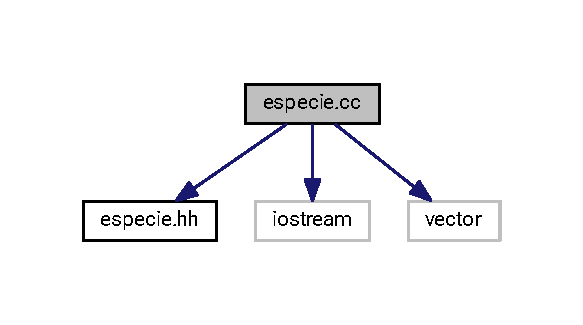
\includegraphics[width=280pt]{especie_8cc__incl}
\end{center}
\end{figure}

\hypertarget{especie_8hh}{}\section{Referència del Fitxer especie.\+hh}
\label{especie_8hh}\index{especie.\+hh@{especie.\+hh}}


Especificació de la clase \hyperlink{especie_8hh}{especie.\+hh}.  


\subsection*{Classes}
\begin{DoxyCompactItemize}
\item 
class \hyperlink{classespecie}{especie}
\begin{DoxyCompactList}\small\item\em Guardem la informacio genetica de la especie. \end{DoxyCompactList}\end{DoxyCompactItemize}


\subsection{Descripció Detallada}
Especificació de la clase \hyperlink{especie_8hh}{especie.\+hh}. 


\hypertarget{individu_8cc}{}\section{Referència del Fitxer individu.\+cc}
\label{individu_8cc}\index{individu.\+cc@{individu.\+cc}}


Codi de la clase individu.  


Inclou el graf de dependències per a individu.\+cc\+:
\nopagebreak
\begin{figure}[H]
\begin{center}
\leavevmode
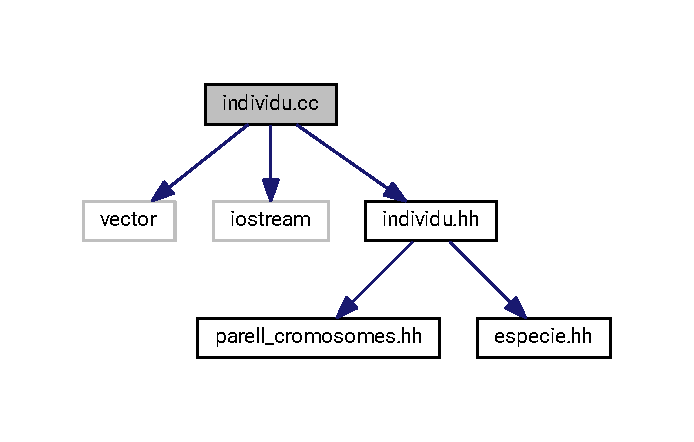
\includegraphics[width=278pt]{individu_8cc__incl}
\end{center}
\end{figure}


\subsection{Descripció Detallada}
Codi de la clase individu. 


\hypertarget{individu_8hh}{}\section{Referència del Fitxer individu.\+hh}
\label{individu_8hh}\index{individu.\+hh@{individu.\+hh}}
Inclou el graf de dependències per a individu.\+hh\+:
\nopagebreak
\begin{figure}[H]
\begin{center}
\leavevmode
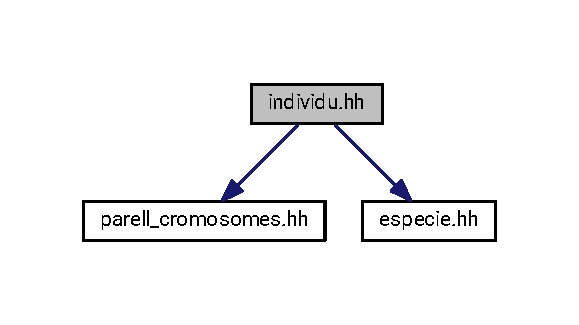
\includegraphics[width=278pt]{individu_8hh__incl}
\end{center}
\end{figure}
\subsection*{Classes}
\begin{DoxyCompactItemize}
\item 
class \hyperlink{classindividu}{individu}
\end{DoxyCompactItemize}
\subsection*{Definicions de Tipus}
\begin{DoxyCompactItemize}
\item 
typedef set$<$ \hyperlink{classindividu}{individu} $>$ \hyperlink{individu_8hh_a32dbccbf05588c8c12b0111d5c5c6eb3}{setiterator}
\end{DoxyCompactItemize}


\subsection{Documentació de les Definicions de Tipus}
\index{individu.\+hh@{individu.\+hh}!setiterator@{setiterator}}
\index{setiterator@{setiterator}!individu.\+hh@{individu.\+hh}}
\subsubsection[{\texorpdfstring{setiterator}{setiterator}}]{\setlength{\rightskip}{0pt plus 5cm}typedef set$<${\bf individu}$>$ {\bf setiterator}}\hypertarget{individu_8hh_a32dbccbf05588c8c12b0111d5c5c6eb3}{}\label{individu_8hh_a32dbccbf05588c8c12b0111d5c5c6eb3}


Definició a la línia 11 del fitxer individu.\+hh.


\hypertarget{parell__cromosomes_8cc}{}\section{Referencia del Archivo parell\+\_\+cromosomes.\+cc}
\label{parell__cromosomes_8cc}\index{parell\+\_\+cromosomes.\+cc@{parell\+\_\+cromosomes.\+cc}}
Dependencia gráfica adjunta para parell\+\_\+cromosomes.\+cc\+:\nopagebreak
\begin{figure}[H]
\begin{center}
\leavevmode
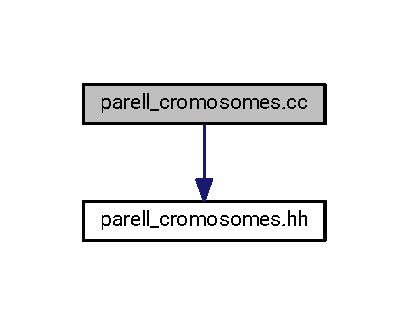
\includegraphics[width=196pt]{parell__cromosomes_8cc__incl}
\end{center}
\end{figure}

\hypertarget{parell__cromosomes_8hh}{}\section{Referència del Fitxer parell\+\_\+cromosomes.\+hh}
\label{parell__cromosomes_8hh}\index{parell\+\_\+cromosomes.\+hh@{parell\+\_\+cromosomes.\+hh}}


Especificació de la clase \hyperlink{classparell__cromosomes}{parell\+\_\+cromosomes}.  


Inclou el graf de dependències per a parell\+\_\+cromosomes.\+hh\+:\nopagebreak
\begin{figure}[H]
\begin{center}
\leavevmode
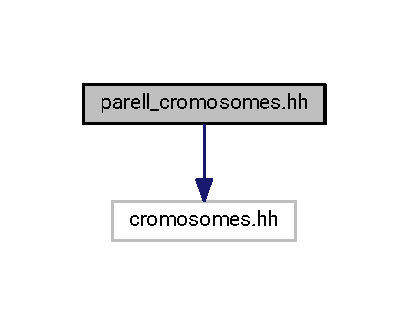
\includegraphics[width=196pt]{parell__cromosomes_8hh__incl}
\end{center}
\end{figure}
\subsection*{Classes}
\begin{DoxyCompactItemize}
\item 
class \hyperlink{classparell__cromosomes}{parell\+\_\+cromosomes}
\end{DoxyCompactItemize}


\subsection{Descripció Detallada}
Especificació de la clase \hyperlink{classparell__cromosomes}{parell\+\_\+cromosomes}. 


\hypertarget{poblacio_8cc}{}\section{Referència del Fitxer poblacio.\+cc}
\label{poblacio_8cc}\index{poblacio.\+cc@{poblacio.\+cc}}


Codi de la clase poblacio.  


Inclou el graf de dependències per a poblacio.\+cc\+:
\nopagebreak
\begin{figure}[H]
\begin{center}
\leavevmode
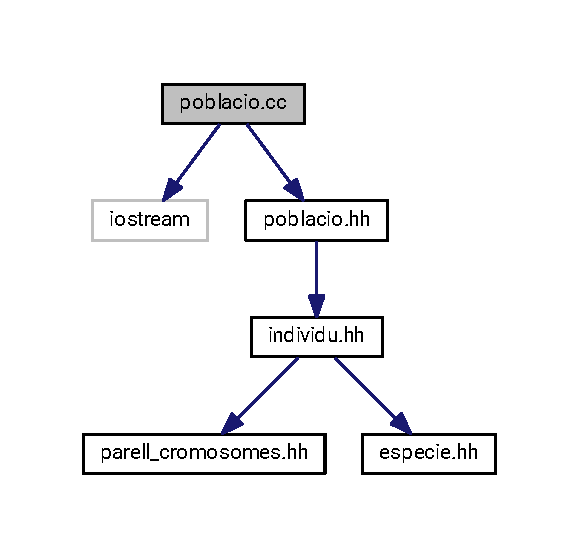
\includegraphics[width=278pt]{poblacio_8cc__incl}
\end{center}
\end{figure}


\subsection{Descripció Detallada}
Codi de la clase poblacio. 


\hypertarget{poblacio_8hh}{}\section{Referència del Fitxer poblacio.\+hh}
\label{poblacio_8hh}\index{poblacio.\+hh@{poblacio.\+hh}}
Inclou el graf de dependències per a poblacio.\+hh\+:
\nopagebreak
\begin{figure}[H]
\begin{center}
\leavevmode
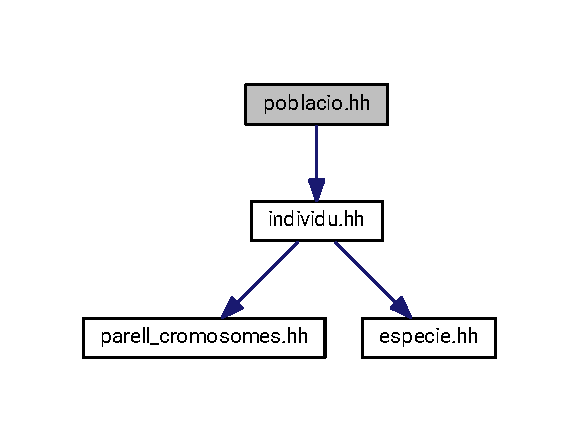
\includegraphics[width=289pt]{poblacio_8hh__incl}
\end{center}
\end{figure}
\subsection*{Classes}
\begin{DoxyCompactItemize}
\item 
class \hyperlink{classpoblacio}{poblacio}
\end{DoxyCompactItemize}

\hypertarget{program_8cc}{}\section{Referencia del Archivo program.\+cc}
\label{program_8cc}\index{program.\+cc@{program.\+cc}}
Dependencia gráfica adjunta para program.\+cc\+:\nopagebreak
\begin{figure}[H]
\begin{center}
\leavevmode
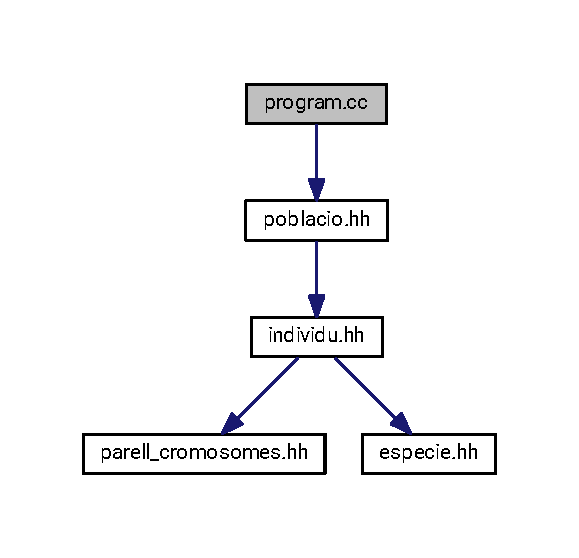
\includegraphics[width=278pt]{program_8cc__incl}
\end{center}
\end{figure}
\subsection*{Enumeraciones}
\subsection*{Funciones}
\begin{DoxyCompactItemize}
\item 
\hyperlink{program_8cc_a7ada6c10a663c040a0822e837b18547c}{string\+\_\+code} \hyperlink{program_8cc_a9b069a6933140b7d05fbc7c0fd8c3f44}{hashit} (string const \&in\+String)
\item 
int \hyperlink{program_8cc_ae66f6b31b5ad750f1fe042a706a4e3d4}{main} ()
\end{DoxyCompactItemize}


\subsection{Documentación de las enumeraciones}
\index{program.\+cc@{program.\+cc}!string\+\_\+code@{string\+\_\+code}}
\index{string\+\_\+code@{string\+\_\+code}!program.\+cc@{program.\+cc}}
\subsubsection[{\texorpdfstring{string\+\_\+code}{string_code}}]{\setlength{\rightskip}{0pt plus 5cm}enum {\bf string\+\_\+code}}\hypertarget{program_8cc_a7ada6c10a663c040a0822e837b18547c}{}\label{program_8cc_a7ada6c10a663c040a0822e837b18547c}
\begin{Desc}
\item[Valores de enumeraciones]\par
\begin{description}
\index{add\+In@{add\+In}!program.\+cc@{program.\+cc}}\index{program.\+cc@{program.\+cc}!add\+In@{add\+In}}\item[{\em 
add\+In\hypertarget{program_8cc_a7ada6c10a663c040a0822e837b18547ca17fa90d3986724847d45c9a4a2950c8c}{}\label{program_8cc_a7ada6c10a663c040a0822e837b18547ca17fa90d3986724847d45c9a4a2950c8c}
}]\index{reproduccion@{reproduccion}!program.\+cc@{program.\+cc}}\index{program.\+cc@{program.\+cc}!reproduccion@{reproduccion}}\item[{\em 
reproduccion\hypertarget{program_8cc_a7ada6c10a663c040a0822e837b18547cad8025600f8b4ac793096ffbb86ede666}{}\label{program_8cc_a7ada6c10a663c040a0822e837b18547cad8025600f8b4ac793096ffbb86ede666}
}]\index{escribir\+\_\+arbol@{escribir\+\_\+arbol}!program.\+cc@{program.\+cc}}\index{program.\+cc@{program.\+cc}!escribir\+\_\+arbol@{escribir\+\_\+arbol}}\item[{\em 
escribir\+\_\+arbol\hypertarget{program_8cc_a7ada6c10a663c040a0822e837b18547caf134679f23751d3e201a28f1d91bb510}{}\label{program_8cc_a7ada6c10a663c040a0822e837b18547caf134679f23751d3e201a28f1d91bb510}
}]\index{completar\+\_\+arbol@{completar\+\_\+arbol}!program.\+cc@{program.\+cc}}\index{program.\+cc@{program.\+cc}!completar\+\_\+arbol@{completar\+\_\+arbol}}\item[{\em 
completar\+\_\+arbol\hypertarget{program_8cc_a7ada6c10a663c040a0822e837b18547ca5679999c4825be93fc15cc050aecbd29}{}\label{program_8cc_a7ada6c10a663c040a0822e837b18547ca5679999c4825be93fc15cc050aecbd29}
}]\index{escribir\+\_\+pob@{escribir\+\_\+pob}!program.\+cc@{program.\+cc}}\index{program.\+cc@{program.\+cc}!escribir\+\_\+pob@{escribir\+\_\+pob}}\item[{\em 
escribir\+\_\+pob\hypertarget{program_8cc_a7ada6c10a663c040a0822e837b18547ca6fad81eec3fd3406a0b163706f3ea859}{}\label{program_8cc_a7ada6c10a663c040a0822e837b18547ca6fad81eec3fd3406a0b163706f3ea859}
}]\index{escribir\+\_\+gen@{escribir\+\_\+gen}!program.\+cc@{program.\+cc}}\index{program.\+cc@{program.\+cc}!escribir\+\_\+gen@{escribir\+\_\+gen}}\item[{\em 
escribir\+\_\+gen\hypertarget{program_8cc_a7ada6c10a663c040a0822e837b18547cacd3c3bb703937d5a2c045b03ef706efb}{}\label{program_8cc_a7ada6c10a663c040a0822e837b18547cacd3c3bb703937d5a2c045b03ef706efb}
}]\index{def@{def}!program.\+cc@{program.\+cc}}\index{program.\+cc@{program.\+cc}!def@{def}}\item[{\em 
def\hypertarget{program_8cc_a7ada6c10a663c040a0822e837b18547ca0b1e0a3345b929f54aedb7a8aaa2c746}{}\label{program_8cc_a7ada6c10a663c040a0822e837b18547ca0b1e0a3345b929f54aedb7a8aaa2c746}
}]\end{description}
\end{Desc}


Definición en la línea 3 del archivo program.\+cc.


\begin{DoxyCode}
3                 \{
4     \hyperlink{program_8cc_a7ada6c10a663c040a0822e837b18547ca17fa90d3986724847d45c9a4a2950c8c}{addIn},
5     \hyperlink{program_8cc_a7ada6c10a663c040a0822e837b18547cad8025600f8b4ac793096ffbb86ede666}{reproduccion},
6     \hyperlink{program_8cc_a7ada6c10a663c040a0822e837b18547caf134679f23751d3e201a28f1d91bb510}{escribir\_arbol},
7     \hyperlink{program_8cc_a7ada6c10a663c040a0822e837b18547ca5679999c4825be93fc15cc050aecbd29}{completar\_arbol},
8     \hyperlink{program_8cc_a7ada6c10a663c040a0822e837b18547ca6fad81eec3fd3406a0b163706f3ea859}{escribir\_pob},
9     \hyperlink{program_8cc_a7ada6c10a663c040a0822e837b18547cacd3c3bb703937d5a2c045b03ef706efb}{escribir\_gen},
10     \hyperlink{program_8cc_a7ada6c10a663c040a0822e837b18547ca0b1e0a3345b929f54aedb7a8aaa2c746}{def}
11 \};
\end{DoxyCode}


\subsection{Documentación de las funciones}
\index{program.\+cc@{program.\+cc}!hashit@{hashit}}
\index{hashit@{hashit}!program.\+cc@{program.\+cc}}
\subsubsection[{\texorpdfstring{hashit(string const \&in\+String)}{hashit(string const &inString)}}]{\setlength{\rightskip}{0pt plus 5cm}{\bf string\+\_\+code} hashit (
\begin{DoxyParamCaption}
\item[{string const \&}]{in\+String}
\end{DoxyParamCaption}
)}\hypertarget{program_8cc_a9b069a6933140b7d05fbc7c0fd8c3f44}{}\label{program_8cc_a9b069a6933140b7d05fbc7c0fd8c3f44}


Definición en la línea 13 del archivo program.\+cc.


\begin{DoxyCode}
13                                             \{
14   cout<<inString;
15     \textcolor{keywordflow}{if} (inString == \textcolor{stringliteral}{"anadir\_individuo"}) \textcolor{keywordflow}{return} \hyperlink{program_8cc_a7ada6c10a663c040a0822e837b18547ca17fa90d3986724847d45c9a4a2950c8c}{addIn};
16     \textcolor{keywordflow}{if} (inString == \textcolor{stringliteral}{"reproduccion\_sexual"}) \textcolor{keywordflow}{return} \hyperlink{program_8cc_a7ada6c10a663c040a0822e837b18547cad8025600f8b4ac793096ffbb86ede666}{reproduccion};
17     \textcolor{keywordflow}{if} (inString == \textcolor{stringliteral}{"escribir\_arbol\_genealogico"}) \textcolor{keywordflow}{return} \hyperlink{program_8cc_a7ada6c10a663c040a0822e837b18547caf134679f23751d3e201a28f1d91bb510}{escribir\_arbol};
18     \textcolor{keywordflow}{if} (inString == \textcolor{stringliteral}{"completar\_arbol\_genealogico"}) \textcolor{keywordflow}{return} \hyperlink{program_8cc_a7ada6c10a663c040a0822e837b18547ca5679999c4825be93fc15cc050aecbd29}{completar\_arbol};
19     \textcolor{keywordflow}{if} (inString == \textcolor{stringliteral}{"escribir\_poblacion"}) \textcolor{keywordflow}{return} \hyperlink{program_8cc_a7ada6c10a663c040a0822e837b18547ca6fad81eec3fd3406a0b163706f3ea859}{escribir\_pob};
20     \textcolor{keywordflow}{if} (inString == \textcolor{stringliteral}{"escribir\_genotipo"}) \textcolor{keywordflow}{return} \hyperlink{program_8cc_a7ada6c10a663c040a0822e837b18547cacd3c3bb703937d5a2c045b03ef706efb}{escribir\_gen};
21     \textcolor{keywordflow}{return} \hyperlink{program_8cc_a7ada6c10a663c040a0822e837b18547ca0b1e0a3345b929f54aedb7a8aaa2c746}{def};
22 \}
\end{DoxyCode}
\index{program.\+cc@{program.\+cc}!main@{main}}
\index{main@{main}!program.\+cc@{program.\+cc}}
\subsubsection[{\texorpdfstring{main()}{main()}}]{\setlength{\rightskip}{0pt plus 5cm}int main (
\begin{DoxyParamCaption}
{}
\end{DoxyParamCaption}
)}\hypertarget{program_8cc_ae66f6b31b5ad750f1fe042a706a4e3d4}{}\label{program_8cc_ae66f6b31b5ad750f1fe042a706a4e3d4}


Definición en la línea 25 del archivo program.\+cc.


\begin{DoxyCode}
25           \{
26     \hyperlink{classespecie}{especie} esp;
27     esp.\hyperlink{classespecie_af1a08ff40fdb79abb1d78c06b8131306}{llegir}();
28     \hyperlink{classpoblacio}{poblacio} pob;
29     pob.\hyperlink{classpoblacio_a02fda63e8b0144ce197764753778a201}{llegir}(esp);
30     \textcolor{keywordtype}{string} op;
31     cin>>op;
32 
33     \textcolor{keywordflow}{while}(op != \textcolor{stringliteral}{"acabar"})\{
34         \textcolor{keywordflow}{switch}(\hyperlink{program_8cc_a9b069a6933140b7d05fbc7c0fd8c3f44}{hashit}(op))\{
35             \textcolor{keywordflow}{case} \hyperlink{program_8cc_a7ada6c10a663c040a0822e837b18547ca17fa90d3986724847d45c9a4a2950c8c}{addIn}:\{  \textcolor{comment}{//funciona !:)}
36                 \textcolor{keywordtype}{string} name;
37                 cin>>name;
38                 cout<<\textcolor{stringliteral}{" "}<<name<<endl;
39                 \hyperlink{classindividu}{individu} in;
40                 in.\hyperlink{classindividu_a6cfcb4f2472be86eb3416da90dc721be}{llegir}(esp);
41                 \textcolor{keywordflow}{if}(pob.\hyperlink{classpoblacio_a9c6fe58f2cbd06574070df2ef4076015}{esta\_individu}(name)) cout<<\textcolor{stringliteral}{"  error"}<<endl;
42                 \textcolor{keywordflow}{else} pob.\hyperlink{classpoblacio_a09a516141a9a8bef9249239916894af5}{afegir\_individu}(name, in);
43 
44                 \textcolor{keywordflow}{break};
45             \}
46             \textcolor{keywordflow}{case} \hyperlink{program_8cc_a7ada6c10a663c040a0822e837b18547cad8025600f8b4ac793096ffbb86ede666}{reproduccion}:\{
47                 \textcolor{keywordtype}{string} mare, pare, fil;  \textcolor{comment}{//funciona !:)}
48                 cin>>mare>>pare>>fil;
49                 cout<<\textcolor{stringliteral}{" "}<<mare<<\textcolor{stringliteral}{" "}<<pare<<\textcolor{stringliteral}{" "}<<fil<<endl;
50                 pob.\hyperlink{classpoblacio_a347bc063088e161813c257211d8059b9}{reproduir}(pare, mare, fil, esp);
51                 \textcolor{keywordflow}{break};
52             \}
53             \textcolor{keywordflow}{case} \hyperlink{program_8cc_a7ada6c10a663c040a0822e837b18547caf134679f23751d3e201a28f1d91bb510}{escribir\_arbol}:\{  \textcolor{comment}{//funciona !:)}
54                 \textcolor{keywordtype}{string} nom;
55                 cin>>nom;
56                 cout<<\textcolor{stringliteral}{" "}<<nom<<endl;
57                 \textcolor{keywordflow}{if}(pob.\hyperlink{classpoblacio_a9c6fe58f2cbd06574070df2ef4076015}{esta\_individu}(nom)) pob.
      \hyperlink{classpoblacio_a30e1c829999a403012ce09172461d656}{escriure\_arbre\_geneologic}(nom);
58                 \textcolor{keywordflow}{else} cout<<\textcolor{stringliteral}{"  error"}<<endl;
59                 \textcolor{keywordflow}{break};
60             \}
61             \textcolor{keywordflow}{case} \hyperlink{program_8cc_a7ada6c10a663c040a0822e837b18547ca5679999c4825be93fc15cc050aecbd29}{completar\_arbol}:\{
62                 pob.\hyperlink{classpoblacio_a1e30be9019dcb194171228c41284117f}{completar\_arbre}();
63                 \textcolor{keywordflow}{break};
64            \}
65             \textcolor{keywordflow}{case} \hyperlink{program_8cc_a7ada6c10a663c040a0822e837b18547ca6fad81eec3fd3406a0b163706f3ea859}{escribir\_pob}:\{  \textcolor{comment}{//funciona !:)}
66                 cout<<endl;
67                 pob.\hyperlink{classpoblacio_aef82aca848d299bc5eff6d6b479a5081}{escriure}();
68                 \textcolor{keywordflow}{break};
69            \}
70             \textcolor{keywordflow}{case} \hyperlink{program_8cc_a7ada6c10a663c040a0822e837b18547cacd3c3bb703937d5a2c045b03ef706efb}{escribir\_gen}:\{  \textcolor{comment}{//funciona !:)}
71                 \textcolor{keywordtype}{string} nom;
72                 cin>>nom;
73                 cout<<\textcolor{stringliteral}{" "}<<nom<<endl;
74                 \textcolor{keywordflow}{if}(pob.\hyperlink{classpoblacio_a9c6fe58f2cbd06574070df2ef4076015}{esta\_individu}(nom)) pob.\hyperlink{classpoblacio_a30ec7988306978a608ab11062069e6e1}{consultar\_individu}(nom).
      \hyperlink{classindividu_a8e9d5b4698e9d2d1838e5a512206768a}{escriure\_genotip}();
75                 \textcolor{keywordflow}{else} cout<<\textcolor{stringliteral}{"  error"}<<endl;
76                 \textcolor{keywordflow}{break};
77           \}
78            \textcolor{keywordflow}{default}:
79                 \textcolor{keywordflow}{break};
80 
81       \}
82       cin>>op;
83   \}
84   cout<<\textcolor{stringliteral}{"acabar"}<<endl;
85 \}
\end{DoxyCode}

%--- End generated contents ---

% Index
\backmatter
\newpage
\phantomsection
\clearemptydoublepage
\addcontentsline{toc}{chapter}{Índice}
\printindex

\end{document}
